% Generated human-review packet template.  Source records, Lean statements,
% and raw-source-to-Spec screening fields are substituted by
% scripts/review_dashboard_packet.py.
% Do not hand-edit generated packets; annotate the PDF or reconcile notes into
% the paper-local human-review log.
\documentclass[10pt]{article}
\usepackage[margin=0.43in]{geometry}
\usepackage{fontspec}
% Use a Unicode-complete main face as well as a Unicode-complete code face.
% Reviewer reasons and source labels can contain exact Greek symbols outside
% verbatim blocks; silently dropping one would corrupt the review packet.
\setmainfont{DejaVu Serif}
% The broad DejaVu Sans Unicode coverage preserves Lean's mathematical glyphs
% (including U+2216 set difference and superscript identifiers) in verbatim
% review blocks.  Its proportional metrics are preferable to silently missing
% exact semantic text from a narrower monospace font.
\setmonofont{DejaVu Sans}
\usepackage{hyperref}
\usepackage{amssymb}
\usepackage{fvextra}
\usepackage{enumitem}
\setlength{\parindent}{0pt}
\setlength{\parskip}{0.15em}
\linespread{0.92}
\hypersetup{colorlinks=true,linkcolor=blue,urlcolor=blue,breaklinks=true}
\DefineVerbatimEnvironment{ReviewVerbatim}{Verbatim}{breaklines=true,breakanywhere=true,fontsize=\scriptsize}
\newcommand{\reviewerbox}{%
  \par\noindent\fbox{\parbox{0.96\linewidth}{\rule{0pt}{0.38in}}}\par
}
\newcommand{\reviewmatch}[1]{%
  \par\noindent\textbf{Reviewer check:} $\square$\; #1\par
  \noindent\emph{If left unchecked, explain the discrepancy or uncertainty below.}\par
}

\begin{document}
\fontsize{9}{10}\selectfont

\begin{center}
{\LARGE Human review packet: GKP26LinearRepresentationHypothesis}\\[0.35em]
\small Generated from byte-pinned source excerpts, the expanded PaperInterface
specifications, and hash-bound raw-source-to-Spec screening records.
\end{center}

\noindent\textbf{Paper:} GKP26LinearRepresentationHypothesis\\
\textbf{Paper id:} \texttt{GKP26LinearRepresentationHypothesis}\\
\textbf{Source version:} \parbox[t]{0.76\linewidth}{\raggedright arXiv v1, 2026}\\
\textbf{Source record:} \texttt{audit/paper\_statement\_map.json}\\
\textbf{Rows:} 11\\
\textbf{Generated:} 2026-09-06\\
\textbf{Source URL:} \href{https://arxiv.org/abs/2602.11246}{official source}





\section*{How to use this packet}
For each source claim, compare the exact source excerpts with the expanded
PaperInterface specification. Mark up this PDF or fill the blank reviewer box in the TeX source;
return the annotated file for reconciliation into the paper-local human-review
log.

\section*{Open the interactive dashboard}
The interactive dashboard is an optional alternative to using this PDF; it
presents the same review surface rather than an additional review requirement.
After forking and cloning (or pulling) AppliedModelingLib, run the following from the
repository root. The cache command is needed only the first time in a new clone.
\begin{ReviewVerbatim}
cd <your-repository-checkout>
lake exe cache get
python3 scripts/review_dashboard.py --paper GKP26LinearRepresentationHypothesis --serve
\end{ReviewVerbatim}
Open \url{http://127.0.0.1:8765/} in a browser and keep that terminal running
while reviewing. The dashboard records saved annotations in this paper's local
reviewer-owned review record.

\section*{Contents}
\begin{itemize}[leftmargin=1.2em]
\item \hyperlink{library-section-394e2d3089a4790e}{Semantic library prerequisites (21; not paper claims)}
\begin{itemize}[leftmargin=1.2em]
\item \hyperlink{library-prerequisite-3b4037efd2578d57}{AppliedModelingLib.\allowbreak{}FairCoin.\allowbreak{}fairMeasure}
\item \hyperlink{library-prerequisite-1ffe905ac568fe34}{AppliedModelingLib.\allowbreak{}FairCoin.\allowbreak{}productMeasure}
\item \hyperlink{library-prerequisite-3d99a970244a38c7}{AppliedModelingLib.\allowbreak{}FiniteDimensionalNorms.\allowbreak{}l1}
\item \hyperlink{library-prerequisite-634c9de2aa959a7a}{AppliedModelingLib.\allowbreak{}FiniteDimensionalNorms.\allowbreak{}l2Sq}
\item \hyperlink{library-prerequisite-08313452edb53fe9}{AppliedModelingLib.\allowbreak{}FiniteDimensionalNorms.\allowbreak{}l2}
\item \hyperlink{library-prerequisite-c35e4379972ea6a7}{AppliedModelingLib.\allowbreak{}Math.\allowbreak{}LinearCompressedSensing.\allowbreak{}InUnitBox}
\item \hyperlink{library-prerequisite-6acf02dccc761051}{AppliedModelingLib.\allowbreak{}Math.\allowbreak{}LinearCompressedSensing.\allowbreak{}InZeroOne}
\item \hyperlink{library-prerequisite-e73f6892dab51ea6}{AppliedModelingLib.\allowbreak{}Math.\allowbreak{}LinearCompressedSensing.\allowbreak{}support}
\item \hyperlink{library-prerequisite-16b52186f2356e0f}{AppliedModelingLib.\allowbreak{}Math.\allowbreak{}LinearCompressedSensing.\allowbreak{}KSparse}
\item \hyperlink{library-prerequisite-80b8245a943a9126}{AppliedModelingLib.\allowbreak{}Math.\allowbreak{}LinearCompressedSensing.\allowbreak{}inner}
\item \hyperlink{library-prerequisite-3c53e0c4df04cc38}{AppliedModelingLib.\allowbreak{}Math.\allowbreak{}LinearCompressedSensing.\allowbreak{}linearProbe}
\item \hyperlink{library-prerequisite-42ffb876520532f3}{AppliedModelingLib.\allowbreak{}Math.\allowbreak{}LinearCompressedSensing.\allowbreak{}SupErrorLt}
\item \hyperlink{library-prerequisite-20e33ca499f2a3dc}{AppliedModelingLib.\allowbreak{}Math.\allowbreak{}LinearCompressedSensing.\allowbreak{}ThresholdSeparates}
\item \hyperlink{library-prerequisite-aa1a79d83728d01e}{AppliedModelingLib.\allowbreak{}Math.\allowbreak{}LinearCompressedSensing.\allowbreak{}vectorNorm}
\item \hyperlink{library-prerequisite-a38f8c1fe77171c1}{AppliedModelingLib.\allowbreak{}Math.\allowbreak{}LinearCompressedSensing.\allowbreak{}normalizedVector}
\item \hyperlink{library-prerequisite-02a659e52c5db02f}{AppliedModelingLib.\allowbreak{}Math.\allowbreak{}LinearCompressedSensing.\allowbreak{}vectorCorrelation}
\item \hyperlink{library-prerequisite-639d1d3f23451e62}{AppliedModelingLib.\allowbreak{}Math.\allowbreak{}TendsToZero}
\item \hyperlink{library-prerequisite-02dcf48d492eec05}{AppliedModelingLib.\allowbreak{}Probability.\allowbreak{}RademacherMatrix.\allowbreak{}rademacherSign}
\item \hyperlink{library-prerequisite-9a1b86b836cebc11}{AppliedModelingLib.\allowbreak{}Probability.\allowbreak{}RademacherMatrix.\allowbreak{}rowsMeasure}
\item \hyperlink{library-prerequisite-afdf9be2af2cdb5d}{AppliedModelingLib.\allowbreak{}Probability.\allowbreak{}RademacherMatrix.\allowbreak{}scaledMatrix}
\item \hyperlink{library-prerequisite-80e84a51ccd3e1cd}{AppliedModelingLib.\allowbreak{}measureProb}
\end{itemize}
\item \hyperlink{paper-prerequisite-section-5ef5ef0364b6939c}{Paper-specific semantic prerequisites (3; not paper claims)}
\begin{itemize}[leftmargin=1.2em]
\item \hyperlink{paper-prerequisite-30c6edfdf8a73952}{GKP26LinearRepresentationHypothesis.\allowbreak{}linearCompressedSensingDimensionValue}
\item \hyperlink{paper-prerequisite-9afe7bd458014ebc}{GKP26LinearRepresentationHypothesis.\allowbreak{}linearRecoveryCondition}
\item \hyperlink{paper-prerequisite-5cd9ac228cafd57b}{GKP26LinearRepresentationHypothesis.\allowbreak{}paper\_\allowbreak{}strict\_\allowbreak{}mu\_\allowbreak{}incoherent}
\end{itemize}
\item \hyperlink{source-section-f10b5f68e4acf3dc}{Source claims (11)}
\begin{itemize}[leftmargin=1.2em]
\item \hyperlink{source-claim-202b0f5354c0082d}{paper\_\allowbreak{}compressed\_\allowbreak{}sensing\_\allowbreak{}external\_\allowbreak{}basis\_\allowbreak{}pursuitSpec}
\item \hyperlink{source-claim-5da06a1a773efe05}{paper\_\allowbreak{}geometry1\_\allowbreak{}source\_\allowbreak{}constructed\_\allowbreak{}rateSpec}
\item \hyperlink{source-claim-0d1630b3f82fa739}{paper\_\allowbreak{}geometry2\_\allowbreak{}probe\_\allowbreak{}column\_\allowbreak{}correlation\_\allowbreak{}upper\_\allowbreak{}correctedSpec}
\item \hyperlink{source-claim-7f9743bbf88fc45a}{paper\_\allowbreak{}geometry2\_\allowbreak{}representation\_\allowbreak{}column\_\allowbreak{}correlation\_\allowbreak{}upper\_\allowbreak{}correctedSpec}
\item \hyperlink{source-claim-93035163b22de06d}{paper\_\allowbreak{}geometry2\_\allowbreak{}self\_\allowbreak{}column\_\allowbreak{}correlation\_\allowbreak{}lowerSpec}
\item \hyperlink{source-claim-a09ca6c3835d7786}{paper\_\allowbreak{}lower\_\allowbreak{}bound\_\allowbreak{}dimension\_\allowbreak{}isBigO\_\allowbreak{}source\_\allowbreak{}log\_\allowbreak{}source\_\allowbreak{}regimeSpec}
\item \hyperlink{source-claim-5793edfccf93335e}{paper\_\allowbreak{}random\_\allowbreak{}rademacher\_\allowbreak{}strict\_\allowbreak{}incoherence\_\allowbreak{}source\_\allowbreak{}rateSpec}
\item \hyperlink{source-claim-c333ecf427637954}{paper\_\allowbreak{}upper\_\allowbreak{}bound\_\allowbreak{}dimension\_\allowbreak{}isBigO\_\allowbreak{}k\_\allowbreak{}sq\_\allowbreak{}log\_\allowbreak{}mSpec}
\item \hyperlink{source-claim-b773a309f631cb95}{paper\_\allowbreak{}rademacher\_\allowbreak{}strict\_\allowbreak{}incoherent\_\allowbreak{}exists\_\allowbreak{}source\_\allowbreak{}rateSpec}
\item \hyperlink{source-claim-b1fd683d79993219}{paper\_\allowbreak{}threshold\_\allowbreak{}separation\_\allowbreak{}dimension\_\allowbreak{}isBigO\_\allowbreak{}lower\_\allowbreak{}source\_\allowbreak{}log\_\allowbreak{}original\_\allowbreak{}regimeSpec}
\item \hyperlink{source-claim-331e1d36e419216b}{paper\_\allowbreak{}activation\_\allowbreak{}separation\_\allowbreak{}dimension\_\allowbreak{}isBigO\_\allowbreak{}lower\_\allowbreak{}source\_\allowbreak{}log\_\allowbreak{}original\_\allowbreak{}regimeSpec}
\end{itemize}
\end{itemize}

\clearpage
\hypertarget{library-section-394e2d3089a4790e}{}
\section*{Material library prerequisites}
\hypertarget{library-prerequisite-3b4037efd2578d57}{}
\subsection*{\small\ttfamily\raggedright AppliedModelingLib.\allowbreak{}FairCoin.\allowbreak{}fairMeasure}
\textbf{Source locator:} {\footnotesize\raggedright cited publication, lines 412-\allowbreak{}418\par}
\paragraph{Verbatim paper-source connection}
\begin{ReviewVerbatim}
\begin{lemma}[Incoherence of Random Matrices]\label{prop:incoherent}
    Let $C\in \RR^{d\times m}$ be a matrix with i.i.d. scaled Rademacher entries $\pm\frac{1}{\sqrt{d}}$. For
    \begin{equation}
        d = O\left(\frac{\log m + \log \frac{1}{\delta}}{\mu^2}\right),
    \end{equation}
    $C$ is $\mu$-incoherent with probability at least $1 - \delta$.
\end{lemma}
\end{ReviewVerbatim}



\paragraph{Lean-expanded library semantic target}
\begin{ReviewVerbatim}
type:
MeasureTheory.Measure Bool

value:
(PMF.bernoulli (1 / 2) AppliedModelingLib.FairCoin.fairMeasure._proof_2).toMeasure
\end{ReviewVerbatim}

\paragraph{Exact Lean library declaration}
\begin{ReviewVerbatim}
noncomputable def fairMeasure : Measure Bool :=
  ((PMF.bernoulli (1 / 2 : NNReal) (by norm_num)).toMeasure : Measure Bool)
\end{ReviewVerbatim}

\paragraph{Recorded source-to-library screening}
\textbf{Verdict:} \texttt{matches}
\\
{\raggedright
\textbf{Reason:} The pinned random-\allowbreak{}matrix proof uses independent uniform signs in \{-\allowbreak{}1,1\};\allowbreak{} fairMeasure is the exact finite sign law used to express one such Rademacher coordinate.\allowbreak{}
\par}
\reviewmatch{Matches source input}
\noindent\textbf{Reviewer annotation}\par
\reviewerbox
\clearpage
\hypertarget{library-prerequisite-1ffe905ac568fe34}{}
\subsection*{\small\ttfamily\raggedright AppliedModelingLib.\allowbreak{}FairCoin.\allowbreak{}productMeasure}
\textbf{Source locator:} {\footnotesize\raggedright cited publication, lines 412-\allowbreak{}418\par}
\paragraph{Verbatim paper-source connection}
\begin{ReviewVerbatim}
\begin{lemma}[Incoherence of Random Matrices]\label{prop:incoherent}
    Let $C\in \RR^{d\times m}$ be a matrix with i.i.d. scaled Rademacher entries $\pm\frac{1}{\sqrt{d}}$. For
    \begin{equation}
        d = O\left(\frac{\log m + \log \frac{1}{\delta}}{\mu^2}\right),
    \end{equation}
    $C$ is $\mu$-incoherent with probability at least $1 - \delta$.
\end{lemma}
\end{ReviewVerbatim}



\paragraph{Lean-expanded library semantic target}
\begin{ReviewVerbatim}
type:
(ι : Type u_1) → MeasureTheory.Measure (ι → Bool)

value:
fun (ι : Type u_1) => MeasureTheory.Measure.infinitePi fun (x : ι) => AppliedModelingLib.FairCoin.fairMeasure
\end{ReviewVerbatim}

\paragraph{Exact Lean library declaration}
\begin{ReviewVerbatim}
noncomputable def productMeasure (ι : Type*) : Measure (ι → Bool) :=
  Measure.infinitePi (fun _ : ι => fairMeasure)
\end{ReviewVerbatim}

\paragraph{Recorded source-to-library screening}
\textbf{Verdict:} \texttt{matches}
\\
{\raggedright
\textbf{Reason:} The pinned proof requires independent Rademacher entries across rows and columns;\allowbreak{} productMeasure is the finite product construction of that stated joint law.\allowbreak{}
\par}
\reviewmatch{Matches source input}
\noindent\textbf{Reviewer annotation}\par
\reviewerbox
\clearpage
\hypertarget{library-prerequisite-3d99a970244a38c7}{}
\subsection*{\small\ttfamily\raggedright AppliedModelingLib.\allowbreak{}FiniteDimensionalNorms.\allowbreak{}l1}
\textbf{Source locator:} {\footnotesize\raggedright cited publication, lines 184-\allowbreak{}199\par}
\paragraph{Verbatim paper-source connection}
\begin{ReviewVerbatim}
Let us recall a classical result in compressed sensing \citep{candes2006near, candes2006robust, donoho2006compressed}, which exactly deals with the setting in which features are represented linearly but accessed non-linearly, answering Q1.
\begin{theorem}[Compressed Sensing]\label{thm:compressed-sensing}
    There exists a matrix $A\in \RR^{d\times m}$ with $d = O\left(k\log \frac{m}{k}\right)$
    such that for all $k$-sparse $z\in \RR^m$,
    \begin{equation}
        g(x) := \argmin_{z'\in \RR^m: x=Az'} \norm{z'}_1
    \end{equation}
    satisfies
    \begin{equation}
        g(Az) = z.
    \end{equation}
\end{theorem}

This shows that when
\begin{equation}
    d = O\left(k\log \frac{m}{k}\right),
\end{ReviewVerbatim}

% report-context-presentation-sha256: c2a1d00e836fd4ff04738d01fcb25cfb8acf7a372ee2243c7bf6defafaddd1ff
\paragraph{Settled source reading}
Compressed sensing: the checked construction restricts the unstated sparse range to 1 ≤ k and 2k ≤ m.

\paragraph{Lean-expanded library semantic target}
\begin{ReviewVerbatim}
type:
{ι : Type u_1} → [Fintype ι] → (ι → ℝ) → ℝ

value:
fun {ι : Type u_1} [Fintype ι] (x : ι → ℝ) => ∑ i : ι, |x i|
\end{ReviewVerbatim}

\paragraph{Exact Lean library declaration}
\begin{ReviewVerbatim}
/-- Finite-coordinate `L1` quantity, written as a sum of absolute values. -/
def l1 {ι : Type*} [Fintype ι] (x : ι → ℝ) : ℝ :=
  ∑ i : ι, |x i|
\end{ReviewVerbatim}

\paragraph{Recorded source-to-library screening}
\textbf{Verdict:} \texttt{matches}
\\
{\raggedright
\textbf{Reason:} The compressed-\allowbreak{}sensing source minimizes the finite-\allowbreak{}dimensional l1 norm of z'.\allowbreak{} The Lean declaration is exactly the sum over coordinates of |x\_\allowbreak{}i|, which is that l1 objective on R\textasciicircum{}m.\allowbreak{}
\par}
\reviewmatch{Matches source input}
\noindent\textbf{Reviewer annotation}\par
\reviewerbox
\clearpage
\hypertarget{library-prerequisite-634c9de2aa959a7a}{}
\subsection*{\small\ttfamily\raggedright AppliedModelingLib.\allowbreak{}FiniteDimensionalNorms.\allowbreak{}l2Sq}
\textbf{Source locator:} {\footnotesize\raggedright cited publication, lines 638-\allowbreak{}655\par}
\paragraph{Verbatim paper-source connection}
\begin{ReviewVerbatim}
\begin{proposition}\label{prop:geometry-2}
    Consider any constants $\epsilon > 0, \gamma \ge 1$. Then if $\norm{a_i},\norm{b_i} \le \gamma$ for all $i\in [m]$ and
    \begin{equation}
        \norm{B^TAz - z}_\infty < \epsilon
    \end{equation}
    for all $k$-sparse $z\in [-1,1]^m$, it holds that
    \begin{enumerate}
        \item[(i)] $\langle \frac{a_i}{\norm{a_i}}, \frac{b_i}{\norm{b_i}}\rangle \ge \frac{1-\epsilon}{\gamma^2}$ for all $i\in [m],$
        \item[(ii)] $\langle \frac{a_i}{\norm{a_i}}, \frac{a_j}{\norm{a_j}}\rangle \le \frac{\epsilon\gamma^2}{1 - \epsilon} + \sqrt{1 - \frac{(1 - \epsilon)^2}{\gamma^4}}$ for all $i\neq j,$
        \item[(iii)] $\langle \frac{b_i}{\norm{b_i}}, \frac{b_j}{\norm{b_j}}\rangle \le \frac{\epsilon\gamma^2}{1 - \epsilon} + \sqrt{1 - \frac{(1 - \epsilon)^2}{\gamma^4}}$ for all $i\neq j.$
    \end{enumerate}
\end{proposition}

\begin{proof}
    We must have that $\langle a_i, b_i\rangle \ge 1 - \epsilon$ since $\norm{B^TAe_i - e_i}_\infty \le \epsilon$. It follows directly that
    \begin{equation}
       \langle a_i, b_i \rangle > 1 - \epsilon \implies \left\langle\frac{a_i}{\norm{a_i}}, \frac{b_i}{\norm{b_i}}\right\rangle \ge \frac{1-\epsilon}{\gamma^2},
    \end{equation}
\end{ReviewVerbatim}

% report-context-presentation-sha256: 9118162d1076fb5b18327ad389e142612883ff8ebd22eed5cb0f38e1225e79e3
\paragraph{Settled source reading}
Geometry Proposition 2: ε > 0 becomes 0 < ε < 1; the first denominator in parts (ii)/(iii) changes from 1 − ε to (1 − ε)², giving a weaker finite bound.

\paragraph{Lean-expanded library semantic target}
\begin{ReviewVerbatim}
type:
{ι : Type u_1} → [Fintype ι] → (ι → ℝ) → ℝ

value:
fun {ι : Type u_1} [Fintype ι] (x : ι → ℝ) => ∑ i : ι, x i ^ 2
\end{ReviewVerbatim}

\paragraph{Exact Lean library declaration}
\begin{ReviewVerbatim}
/-- Squared finite-coordinate `L2` quantity. -/
def l2Sq {ι : Type*} [Fintype ι] (x : ι → ℝ) : ℝ :=
  ∑ i : ι, x i ^ 2
\end{ReviewVerbatim}

\paragraph{Recorded source-to-library screening}
\textbf{Verdict:} \texttt{matches}
\\
{\raggedright
\textbf{Reason:} The Proposition 2 source uses squared Euclidean column norms through gamma\textasciicircum{}2 and normalized inner products.\allowbreak{} The Lean value sum\_\allowbreak{}i x\_\allowbreak{}i\textasciicircum{}2 is exactly the squared Euclidean norm on the finite coordinate space.\allowbreak{}
\par}
\reviewmatch{Matches source input}
\noindent\textbf{Reviewer annotation}\par
\reviewerbox
\clearpage
\hypertarget{library-prerequisite-08313452edb53fe9}{}
\subsection*{\small\ttfamily\raggedright AppliedModelingLib.\allowbreak{}FiniteDimensionalNorms.\allowbreak{}l2}
\textbf{Source locator:} {\footnotesize\raggedright cited publication, lines 547-\allowbreak{}610\par}
\paragraph{Verbatim paper-source connection}
\begin{ReviewVerbatim}
\begin{proposition}\label{prop:geometry-1}
    Consider constants $\epsilon, \delta\in (0,1)$. Then for $d = O_{\epsilon,\delta}(k^2\log m),$ there exists $A,B\in \RR^{d\times m}$ such that
    \begin{equation}
        \norm{B^TAz - z}_\infty < \epsilon
    \end{equation}
    for all $k$-sparse $z\in [-1,1]^m,$ and where
    \begin{enumerate}
        \item[(i)] $|\langle \frac{a_i}{\norm{a_i}}, \frac{b_i}{\norm{b_i}}\rangle| < \delta + o(1)$ for all $i\in [m]$,
        \item[(ii)] $\langle \frac{a_i}{\norm{a_i}}, \frac{a_j}{\norm{a_j}}\rangle
        > 1 - \delta - o(1)$ for all $i\neq j$,
        \item[(iii)] $\langle \frac{b_i}{\norm{b_i}}, \frac{b_j}{\norm{b_j}}\rangle > 1 - \delta - o(1)$ for all $i\neq j$.
    \end{enumerate}
\end{proposition}

\begin{proof}
    We give a construction. Let $c_1,c_2,\cdots,c_m,a^*,b^*$ be the columns of a $\mu$-incoherent matrix $\RR^{d\times m+2}$. Then set
    \begin{align}
        a_i &= c_i + \lambda a^*\\
        b_i &= c_i + \lambda b^*
    \end{align}
    for $\lambda = \sqrt{\frac{1}{\delta} - 1}.$
    We begin by showing that for an appropriately chosen $\mu$, $\norm{B^TAz - z}_\infty < \epsilon$ for all $k$-sparse $z\in [-1,1]^m.$ Now let $\hat{z} = B^TAz$ for any $z\in [-1,1]^m$ with support $T$. Then
    \begin{equation}
        \hat{z}_i = \left\langle b_i, \sum_{j=1}^m z_ja_j \right\rangle
        = z_i\langle b_i, a_i\rangle + \sum_{j\in T\setminus \{i\}} z_j\langle b_i, a_j\rangle.
    \end{equation}
    Therefore,
    \begin{align}
        |\hat{z}_i - z_i| &\le |z_i(\langle b_i, a_i\rangle - 1)| + \sum_{j\in T\setminus \{i\}} |z_j\langle b_i, a_j\rangle|\\
        &\le |z_i(\langle b_i, a_i \rangle - 1)| + \sum_{j\in T\setminus \{i\}} |\langle b_i, a_j\rangle|,
    \end{align}
    where the last inequality follows from observing that $z_j \in [-1,1]$ for all $j\in [m].$ Now observe that
    \begin{align}
        |z_i(\langle b_i, a_i\rangle - 1)| &= |z_i||\langle c_i + \lambda b^*, c_i + \lambda a^*\rangle - 1|\\
        &\le |z_i|\left(|\langle c_i, \lambda a^*\rangle| + |\langle \lambda b^*, c_i \rangle| + |\langle \lambda b^*, \lambda a^* \rangle|\right) \label{eq:apple-1}\\
        &= |z_i|(2\lambda  + \lambda^2)\mu\label{eq:apple-2}\\
        &< |z_i|(1 + \lambda)^2\mu,
    \end{align}
    where \eqref{eq:apple-1} follows because $|\langle c_i, c_i \rangle| = 1$ and \eqref{eq:apple-2} follows from $\mu$-incoherence. Similarly,
    \begin{align}
        |\langle b_i, a_j\rangle| &= |\langle c_i + \lambda b^*, c_i + \lambda a^*\rangle|\\
        &= |\langle c_i, c_j\rangle| + |\langle c_i, \lambda a^*\rangle| + |\langle \lambda b^*, c_i \rangle| + |\langle \lambda b^*, \lambda a^* \rangle|\\
        &\le (1+2\lambda+\lambda^2)\mu = (1 + \lambda)^2\mu.
    \end{align}
    This implies that
    \begin{equation}
        |z_i(\langle b_i, a_i \rangle - 1)| + \sum_{j\in T\setminus \{i\}} |\langle b_i, a_j\rangle| < k (1 + \lambda)^2\mu,
    \end{equation}
    where we use the fact that if $|z_i| > 0$, then $|T\setminus \{i\}|\le k-1.$ Therefore, it suffices to take $\mu = \frac{\epsilon}{k(1+\lambda^2)}$ to ensure that $\norm{\hat{z}-z}_\infty < \epsilon.$ From \Cref{prop:incoherent}, there exists a $\mu$-incoherent matrix in $\RR^{d\times m+2}$ for
    \begin{equation}
        d = O\left(\frac{k^2(1+\lambda)^4}{\epsilon^2}\log (m+2)\right) = O\left(\frac{k^2(1+\lambda)^4}{\epsilon^2}\log m\right) = O_{\epsilon,\delta}(k^2\log m).
    \end{equation}

    \paragraph{Establishing (i).} We now show that the construction satisfies (i). Observe that for all $i\in [m],$
    \begin{align}
        \left|\left\langle \frac{a_i}{\norm{a_i}}, \frac{b_i}{\norm{b_i}} \right\rangle\right|
        &= \frac{|\langle c_i + \lambda a^*, c_i + \lambda b^*\rangle|}{\norm{a_i}\norm{b_i}}\\
        &\le \frac{|\langle c_i, c_i\rangle| + |\langle c_i, \lambda b^*\rangle| + |\langle \lambda a^*, c_i \rangle| + |\langle \lambda a^*, \lambda b^* \rangle|}{\norm{a_i}\norm{b_i}}\\
        &\le \frac{1 + (2\lambda  + \lambda^2)\mu}{\norm{a_i}\norm{b_i}} = \frac{1 + \frac{(2\lambda  + \lambda^2)\epsilon}{k(1+\lambda^2)}}{\norm{a_i}\norm{b_i}} = \frac{1 + o(1)}{\norm{a_i}\norm{b_i}}.\label{eq:dog}
    \end{align}
    Note that
    \begin{align}
        \langle a_i, a_i\rangle &= \langle c_i + \lambda a^*, c_i + \lambda a^* \rangle\\ &= \langle c_i, c_i\rangle + 2\langle c_i, \lambda a^*\rangle + \langle \lambda a^*, \lambda a^*\rangle\\
        &\le 1 + \lambda^2 - 2\lambda\mu =  1 + \lambda^2 - \frac{2\lambda\epsilon}{k(1+\lambda^2)} = 1 + \lambda^2 - o(1).
\end{ReviewVerbatim}



\paragraph{Lean-expanded library semantic target}
\begin{ReviewVerbatim}
type:
{ι : Type u_1} → [Fintype ι] → (ι → ℝ) → ℝ

value:
fun {ι : Type u_1} [Fintype ι] (x : ι → ℝ) => √(AppliedModelingLib.FiniteDimensionalNorms.l2Sq x)
\end{ReviewVerbatim}

\paragraph{Exact Lean library declaration}
\begin{ReviewVerbatim}
/-- Finite-coordinate `L2` quantity, written as the square root of `l2Sq`. -/
def l2 {ι : Type*} [Fintype ι] (x : ι → ℝ) : ℝ :=
  Real.sqrt (l2Sq x)
\end{ReviewVerbatim}

\paragraph{Recorded source-to-library screening}
\textbf{Verdict:} \texttt{matches}
\\
{\raggedright
\textbf{Reason:} Geometry Proposition 1 uses Euclidean column norms.\allowbreak{} The Lean declaration takes the square root of l2Sq, whose displayed value is the finite sum of coordinate squares, exactly the Euclidean norm on R\textasciicircum{}d.\allowbreak{}
\par}
\reviewmatch{Matches source input}
\noindent\textbf{Reviewer annotation}\par
\reviewerbox
\clearpage
\hypertarget{library-prerequisite-c35e4379972ea6a7}{}
\subsection*{\small\ttfamily\raggedright AppliedModelingLib.\allowbreak{}Math.\allowbreak{}LinearCompressedSensing.\allowbreak{}InUnitBox}
\textbf{Source locator:} {\footnotesize\raggedright cited publication, lines 205-\allowbreak{}209\par}
\paragraph{Verbatim paper-source connection}
\begin{ReviewVerbatim}
Let $d(m,k,\epsilon)$ be the smallest choice of $d$ such that there exists $A,B\in \RR^{d\times m}$ such that
\begin{equation}
    \norm{B^TAz - z}_\infty < \epsilon
\end{equation}
for all $k$-sparse $z\in [-1,1]^m$. (Here, any bounded interval would suffice.)

[Next verbatim source excerpt]










\subsection{Intuition and Proof Techniques}
We begin by developing some geometric intuition for the problem. Let $a_1,\cdots,a_m\in \RR^d$ be the columns of $A\in \RR^{d\times m}$ and $b_1,\cdots,b_m\in \RR^d$ be the columns of $B\in \RR^{d\times m}$. For each $i\in [m]$, we recall that $a_i$ is feature $i$'s \textbf{representation vector} and $b_i$ is feature $i$'s \textbf{probe vector}. Now let $\hat{z} = B^TAz.$ We are interested in when
\begin{equation}\label{eq:salmon}
    \norm{\hat{z}-z}_\infty < \epsilon \iff |\hat{z}_i - z_i| < \epsilon,\quad \forall i\in [m].
\end{equation}
Note that
\begin{equation}
\end{ReviewVerbatim}



\paragraph{Lean-expanded library semantic target}
\begin{ReviewVerbatim}
type:
{Feature : Type u_1} → (Feature → ℝ) → Prop

value:
fun {Feature : Type u_1} (z : Feature → ℝ) => ∀ (i : Feature), |z i| ≤ 1
\end{ReviewVerbatim}

\paragraph{Exact Lean library declaration}
\begin{ReviewVerbatim}
/-- Unit-box convention `z in [-1,1]^m`, stated as absolute-value bounds. -/
def InUnitBox (z : Feature → ℝ) : Prop :=
  ∀ i, |z i| ≤ 1
\end{ReviewVerbatim}

\paragraph{Recorded source-to-library screening}
\textbf{Verdict:} \texttt{matches}
\\
{\raggedright
\textbf{Reason:} The source recovery domain is z in [-\allowbreak{}1,1]\textasciicircum{}m.\allowbreak{} The Lean predicate requires |z\_\allowbreak{}i| <= 1 for every feature coordinate, which is exactly membership in that unit box.\allowbreak{}
\par}
\reviewmatch{Matches source input}
\noindent\textbf{Reviewer annotation}\par
\reviewerbox
\clearpage
\hypertarget{library-prerequisite-6acf02dccc761051}{}
\subsection*{\small\ttfamily\raggedright AppliedModelingLib.\allowbreak{}Math.\allowbreak{}LinearCompressedSensing.\allowbreak{}InZeroOne}
\textbf{Source locator:} {\footnotesize\raggedright cited publication, lines 700-\allowbreak{}733\par}
\paragraph{Verbatim paper-source connection}
\begin{ReviewVerbatim}
Here, we prove that when feature representations are restricted to the Boolean cube $\{0,1\}^m,$ $\Omega(k^2\log (m/k))$ embedding dimensions are required to linearly separate embeddings with and without a feature. A corollary is that adding a bias and monotonic activation function does not increase the asymptotic capacity of embeddings.

\begin{theorem}\label{thm:threshold}
    Suppose that there exist $A,B \in \RR^{d\times m}$ and $t\in \RR^m$ such that for all $i\in [m]$ and $k$-sparse $z\in \{0,1\}^m$,
    \begin{equation}\label{eq:pineapple}
        (B^TAz)_i > t_i
    \end{equation}
    if and only if $z_i=1.$ Then for $k < \sqrt{m}$,
    \begin{equation}
        d = \Omega\left(\frac{k^2}{\log k}\log\frac{m}{k}\right).
    \end{equation}
\end{theorem}
It's worth noting here that taking $\epsilon < \frac{1}{2}$ in \Cref{thm:upper} provides a nearly-matching upper bound of $\Omega(k^2\log m)$, since $\epsilon < \frac{1}{2}$ implies that $(B^TAz)_i < \frac{1}{2}$ when $z_i = 0$ and $(B^TAz)_i > \frac{1}{2}$ when $z_i = 1$. Similarly, \Cref{thm:threshold} implies \Cref{thm:lower} in the case $\epsilon < \frac{1}{2}$. However, the lower bound in \Cref{thm:lower} does not directly imply \Cref{thm:threshold} since we do not require that $\norm{B^TAz - z}_\infty$ is small here, but rather that $Az$ linearly separates positive and negative examples for each feature. That being said, the proof is very similar to that of \Cref{thm:lower}, relying on the same overall strategy.

\begin{proof}
    Suppose that there existed $A,B\in \RR^{d\times m}$ and $t\in \RR^m$ such that for all $i\in [m]$ and $k$-sparse $z\in \{0,1\}^m,$ $(B^TAz)_i > t_i$ if and only if $z_i = 1.$ Then notice that we could scale the $i$-th column of $B$ and $\gamma_i$ by any constant positive factor to get another solution. In particular, we can obtain a solution where $B^TA$ is $1$ on the diagonal. Therefore, it suffices to show that for $d \le O(\frac{k^2}{\log k}\log \frac{m}{k}),$ there does not exist $B,A,t$ satisfying \eqref{eq:pineapple} and such that $(B^TA)_{ii} = 1$ for all $i\in [m].$

    Then we have that $t_i \le 1,$ since $(B^TAe_i) > t_i$ Then, along the lines of the proof of \Cref{thm:lower}, it suffices to find $i\in [m]$ and $T^*\subseteq [m]\setminus \{i\}$ with $|T^*|=2k$ and
    \begin{equation}
        |\langle b_i, a_j \rangle| > \frac{1}{k}
    \end{equation}
    for all $j\in T^*$. Indeed, this would imply the existence of a pair $i\in [m], T\subseteq [m]\setminus\{i\}$ (with $|T|=k$), such that
    \begin{equation}
        (B^TAz)_i > k\cdot \frac{1}{k} = 1 \ge t_i,
    \end{equation}
    giving a contradiction.

    We will again apply \Cref{lem:alon} to submatrices of $C$ of size $r$. Indeed, \Cref{lem:alon} implies that there exists a constant $\alpha > 0$ such that if $|R|=r$ and
    \begin{equation}
        \rank(C_R) < \alpha \frac{\log r}{(\frac{1}{k})^2\log k} = \alpha \frac{k^2}{\log k}\log r,
    \end{equation}
    then $C_R$ has an off-diagonal entry with absolute value at least $\frac{1}{k}.$ Then we can proceed as in the proof of \Cref{thm:lower}, taking $r = \frac{m}{4k+1}$ and applying Tur\'an's theorem.
\end{proof}
\end{ReviewVerbatim}



\paragraph{Lean-expanded library semantic target}
\begin{ReviewVerbatim}
type:
{Feature : Type u_1} → (Feature → ℝ) → Prop

value:
fun {Feature : Type u_1} (z : Feature → ℝ) => ∀ (i : Feature), z i = 0 ∨ z i = 1
\end{ReviewVerbatim}

\paragraph{Exact Lean library declaration}
\begin{ReviewVerbatim}
/-- Boolean feature vectors, represented over reals. -/
def InZeroOne (z : Feature → ℝ) : Prop :=
  ∀ i, z i = 0 ∨ z i = 1
\end{ReviewVerbatim}

\paragraph{Recorded source-to-library screening}
\textbf{Verdict:} \texttt{matches}
\\
{\raggedright
\textbf{Reason:} The threshold theorem quantifies over Boolean vectors z in \{0,1\}\textasciicircum{}m.\allowbreak{} The Lean predicate requires every real-\allowbreak{}valued coordinate to equal either 0 or 1, exactly that source domain.\allowbreak{}
\par}
\reviewmatch{Matches source input}
\noindent\textbf{Reviewer annotation}\par
\reviewerbox
\clearpage
\hypertarget{library-prerequisite-e73f6892dab51ea6}{}
\subsection*{\small\ttfamily\raggedright AppliedModelingLib.\allowbreak{}Math.\allowbreak{}LinearCompressedSensing.\allowbreak{}support}
\textbf{Source locator:} {\footnotesize\raggedright cited publication, lines 205-\allowbreak{}209\par}
\paragraph{Verbatim paper-source connection}
\begin{ReviewVerbatim}
Let $d(m,k,\epsilon)$ be the smallest choice of $d$ such that there exists $A,B\in \RR^{d\times m}$ such that
\begin{equation}
    \norm{B^TAz - z}_\infty < \epsilon
\end{equation}
for all $k$-sparse $z\in [-1,1]^m$. (Here, any bounded interval would suffice.)

[Next verbatim source excerpt]










\subsection{Intuition and Proof Techniques}
We begin by developing some geometric intuition for the problem. Let $a_1,\cdots,a_m\in \RR^d$ be the columns of $A\in \RR^{d\times m}$ and $b_1,\cdots,b_m\in \RR^d$ be the columns of $B\in \RR^{d\times m}$. For each $i\in [m]$, we recall that $a_i$ is feature $i$'s \textbf{representation vector} and $b_i$ is feature $i$'s \textbf{probe vector}. Now let $\hat{z} = B^TAz.$ We are interested in when
\begin{equation}\label{eq:salmon}
    \norm{\hat{z}-z}_\infty < \epsilon \iff |\hat{z}_i - z_i| < \epsilon,\quad \forall i\in [m].
\end{equation}
Note that
\begin{equation}
\end{ReviewVerbatim}



\paragraph{Lean-expanded library semantic target}
\begin{ReviewVerbatim}
type:
{Feature : Type u_1} → [Fintype Feature] → [DecidableEq Feature] → (Feature → ℝ) → Finset Feature

value:
fun {Feature : Type u_1} [Fintype Feature] [DecidableEq Feature] (z : Feature → ℝ) => {i : Feature | z i ≠ 0}
\end{ReviewVerbatim}

\paragraph{Exact Lean library declaration}
\begin{ReviewVerbatim}
/-- Nonzero support of a finite real vector. -/
noncomputable def support [Fintype Feature] [DecidableEq Feature]
    (z : Feature → ℝ) : Finset Feature :=
  Finset.univ.filter fun i => z i ≠ 0
\end{ReviewVerbatim}

\paragraph{Recorded source-to-library screening}
\textbf{Verdict:} \texttt{matches}
\\
{\raggedright
\textbf{Reason:} The source notion of k-\allowbreak{}sparsity counts nonzero feature coordinates.\allowbreak{} The Lean support is precisely the finite set of indices i with z\_\allowbreak{}i != 0 on the paper's finite feature set.\allowbreak{}
\par}
\reviewmatch{Matches source input}
\noindent\textbf{Reviewer annotation}\par
\reviewerbox
\clearpage
\hypertarget{library-prerequisite-16b52186f2356e0f}{}
\subsection*{\small\ttfamily\raggedright AppliedModelingLib.\allowbreak{}Math.\allowbreak{}LinearCompressedSensing.\allowbreak{}KSparse}
\textbf{Source locator:} {\footnotesize\raggedright cited publication, lines 205-\allowbreak{}209\par}
\paragraph{Verbatim paper-source connection}
\begin{ReviewVerbatim}
Let $d(m,k,\epsilon)$ be the smallest choice of $d$ such that there exists $A,B\in \RR^{d\times m}$ such that
\begin{equation}
    \norm{B^TAz - z}_\infty < \epsilon
\end{equation}
for all $k$-sparse $z\in [-1,1]^m$. (Here, any bounded interval would suffice.)

[Next verbatim source excerpt]










\subsection{Intuition and Proof Techniques}
We begin by developing some geometric intuition for the problem. Let $a_1,\cdots,a_m\in \RR^d$ be the columns of $A\in \RR^{d\times m}$ and $b_1,\cdots,b_m\in \RR^d$ be the columns of $B\in \RR^{d\times m}$. For each $i\in [m]$, we recall that $a_i$ is feature $i$'s \textbf{representation vector} and $b_i$ is feature $i$'s \textbf{probe vector}. Now let $\hat{z} = B^TAz.$ We are interested in when
\begin{equation}\label{eq:salmon}
    \norm{\hat{z}-z}_\infty < \epsilon \iff |\hat{z}_i - z_i| < \epsilon,\quad \forall i\in [m].
\end{equation}
Note that
\begin{equation}
\end{ReviewVerbatim}



\paragraph{Lean-expanded library semantic target}
\begin{ReviewVerbatim}
type:
{Feature : Type u_1} → [Fintype Feature] → [DecidableEq Feature] → ℕ → (Feature → ℝ) → Prop

value:
fun {Feature : Type u_1} [Fintype Feature] [DecidableEq Feature] (k : ℕ) (z : Feature → ℝ) =>
  (AppliedModelingLib.Math.LinearCompressedSensing.support z).card ≤ k
\end{ReviewVerbatim}

\paragraph{Exact Lean library declaration}
\begin{ReviewVerbatim}
/-- A finite vector is `k`-sparse when its nonzero support has cardinality at most `k`. -/
def KSparse [Fintype Feature] [DecidableEq Feature]
    (k : ℕ) (z : Feature → ℝ) : Prop :=
  (support z).card ≤ k
\end{ReviewVerbatim}

\paragraph{Recorded source-to-library screening}
\textbf{Verdict:} \texttt{matches}
\\
{\raggedright
\textbf{Reason:} The source uses k-\allowbreak{}sparse vectors, meaning at most k nonzero coordinates.\allowbreak{} The Lean predicate requires the displayed nonzero support Finset to have cardinality at most k;\allowbreak{} its finite and decidable-\allowbreak{}equality binders are available on the paper's [m] index set.\allowbreak{}
\par}
\reviewmatch{Matches source input}
\noindent\textbf{Reviewer annotation}\par
\reviewerbox
\clearpage
\hypertarget{library-prerequisite-80b8245a943a9126}{}
\subsection*{\small\ttfamily\raggedright AppliedModelingLib.\allowbreak{}Math.\allowbreak{}LinearCompressedSensing.\allowbreak{}inner}
\textbf{Source locator:} {\footnotesize\raggedright cited publication, lines 638-\allowbreak{}655\par}
\paragraph{Verbatim paper-source connection}
\begin{ReviewVerbatim}
\begin{proposition}\label{prop:geometry-2}
    Consider any constants $\epsilon > 0, \gamma \ge 1$. Then if $\norm{a_i},\norm{b_i} \le \gamma$ for all $i\in [m]$ and
    \begin{equation}
        \norm{B^TAz - z}_\infty < \epsilon
    \end{equation}
    for all $k$-sparse $z\in [-1,1]^m$, it holds that
    \begin{enumerate}
        \item[(i)] $\langle \frac{a_i}{\norm{a_i}}, \frac{b_i}{\norm{b_i}}\rangle \ge \frac{1-\epsilon}{\gamma^2}$ for all $i\in [m],$
        \item[(ii)] $\langle \frac{a_i}{\norm{a_i}}, \frac{a_j}{\norm{a_j}}\rangle \le \frac{\epsilon\gamma^2}{1 - \epsilon} + \sqrt{1 - \frac{(1 - \epsilon)^2}{\gamma^4}}$ for all $i\neq j,$
        \item[(iii)] $\langle \frac{b_i}{\norm{b_i}}, \frac{b_j}{\norm{b_j}}\rangle \le \frac{\epsilon\gamma^2}{1 - \epsilon} + \sqrt{1 - \frac{(1 - \epsilon)^2}{\gamma^4}}$ for all $i\neq j.$
    \end{enumerate}
\end{proposition}

\begin{proof}
    We must have that $\langle a_i, b_i\rangle \ge 1 - \epsilon$ since $\norm{B^TAe_i - e_i}_\infty \le \epsilon$. It follows directly that
    \begin{equation}
       \langle a_i, b_i \rangle > 1 - \epsilon \implies \left\langle\frac{a_i}{\norm{a_i}}, \frac{b_i}{\norm{b_i}}\right\rangle \ge \frac{1-\epsilon}{\gamma^2},
    \end{equation}
\end{ReviewVerbatim}

% report-context-presentation-sha256: 9118162d1076fb5b18327ad389e142612883ff8ebd22eed5cb0f38e1225e79e3
\paragraph{Settled source reading}
Geometry Proposition 2: ε > 0 becomes 0 < ε < 1; the first denominator in parts (ii)/(iii) changes from 1 − ε to (1 − ε)², giving a weaker finite bound.

\paragraph{Lean-expanded library semantic target}
\begin{ReviewVerbatim}
type:
{Coord : Type u_2} → [Fintype Coord] → (Coord → ℝ) → (Coord → ℝ) → ℝ

value:
fun {Coord : Type u_2} [Fintype Coord] (x y : Coord → ℝ) => ∑ r : Coord, x r * y r
\end{ReviewVerbatim}

\paragraph{Exact Lean library declaration}
\begin{ReviewVerbatim}
/-- Finite real inner product written as a sum over coordinates. -/
def inner [Fintype Coord] (x y : Coord → ℝ) : ℝ :=
  ∑ r, x r * y r
\end{ReviewVerbatim}

\paragraph{Recorded source-to-library screening}
\textbf{Verdict:} \texttt{matches}
\\
{\raggedright
\textbf{Reason:} Proposition 2 uses the ordinary real Euclidean inner product of d-\allowbreak{}dimensional columns.\allowbreak{} The Lean declaration is the finite coordinate sum of x\_\allowbreak{}r*y\_\allowbreak{}r, exactly that inner product.\allowbreak{}
\par}
\reviewmatch{Matches source input}
\noindent\textbf{Reviewer annotation}\par
\reviewerbox
\clearpage
\hypertarget{library-prerequisite-3c53e0c4df04cc38}{}
\subsection*{\small\ttfamily\raggedright AppliedModelingLib.\allowbreak{}Math.\allowbreak{}LinearCompressedSensing.\allowbreak{}linearProbe}
\textbf{Source locator:} {\footnotesize\raggedright cited publication, lines 205-\allowbreak{}209\par}
\paragraph{Verbatim paper-source connection}
\begin{ReviewVerbatim}
Let $d(m,k,\epsilon)$ be the smallest choice of $d$ such that there exists $A,B\in \RR^{d\times m}$ such that
\begin{equation}
    \norm{B^TAz - z}_\infty < \epsilon
\end{equation}
for all $k$-sparse $z\in [-1,1]^m$. (Here, any bounded interval would suffice.)

[Next verbatim source excerpt]










\subsection{Intuition and Proof Techniques}
We begin by developing some geometric intuition for the problem. Let $a_1,\cdots,a_m\in \RR^d$ be the columns of $A\in \RR^{d\times m}$ and $b_1,\cdots,b_m\in \RR^d$ be the columns of $B\in \RR^{d\times m}$. For each $i\in [m]$, we recall that $a_i$ is feature $i$'s \textbf{representation vector} and $b_i$ is feature $i$'s \textbf{probe vector}. Now let $\hat{z} = B^TAz.$ We are interested in when
\begin{equation}\label{eq:salmon}
    \norm{\hat{z}-z}_\infty < \epsilon \iff |\hat{z}_i - z_i| < \epsilon,\quad \forall i\in [m].
\end{equation}
Note that
\begin{equation}
\end{ReviewVerbatim}



\paragraph{Lean-expanded library semantic target}
\begin{ReviewVerbatim}
type:
{Feature : Type u_1} →
  {Coord : Type u_2} →
    [Fintype Feature] → [Fintype Coord] → (Feature → Coord → ℝ) → (Feature → Coord → ℝ) → (Feature → ℝ) → Feature → ℝ

value:
fun {Feature : Type u_1} {Coord : Type u_2} [Fintype Feature] [Fintype Coord] (A B : Feature → Coord → ℝ)
    (z : Feature → ℝ) (i : Feature) =>
  ∑ j : Feature, z j * AppliedModelingLib.Math.LinearCompressedSensing.inner (B i) (A j)
\end{ReviewVerbatim}

\paragraph{Exact Lean library declaration}
\begin{ReviewVerbatim}
/-- Coordinate `i` of `B^T A z`, written using representation and probe columns. -/
def linearProbe [Fintype Feature] [Fintype Coord]
    (A B : Feature → Coord → ℝ) (z : Feature → ℝ) (i : Feature) : ℝ :=
  ∑ j, z j * inner (B i) (A j)
\end{ReviewVerbatim}

\paragraph{Recorded source-to-library screening}
\textbf{Verdict:} \texttt{matches}
\\
{\raggedright
\textbf{Reason:} The source defines hat z=B\textasciicircum{}T A z.\allowbreak{} Its i-\allowbreak{}th coordinate is sum\_\allowbreak{}j z\_\allowbreak{}j times the inner product of probe column B\_\allowbreak{}i with representation column A\_\allowbreak{}j, which is exactly the displayed Lean formula.\allowbreak{}
\par}
\reviewmatch{Matches source input}
\noindent\textbf{Reviewer annotation}\par
\reviewerbox
\clearpage
\hypertarget{library-prerequisite-42ffb876520532f3}{}
\subsection*{\small\ttfamily\raggedright AppliedModelingLib.\allowbreak{}Math.\allowbreak{}LinearCompressedSensing.\allowbreak{}SupErrorLt}
\textbf{Source locator:} {\footnotesize\raggedright cited publication, lines 205-\allowbreak{}209\par}
\paragraph{Verbatim paper-source connection}
\begin{ReviewVerbatim}
Let $d(m,k,\epsilon)$ be the smallest choice of $d$ such that there exists $A,B\in \RR^{d\times m}$ such that
\begin{equation}
    \norm{B^TAz - z}_\infty < \epsilon
\end{equation}
for all $k$-sparse $z\in [-1,1]^m$. (Here, any bounded interval would suffice.)

[Next verbatim source excerpt]










\subsection{Intuition and Proof Techniques}
We begin by developing some geometric intuition for the problem. Let $a_1,\cdots,a_m\in \RR^d$ be the columns of $A\in \RR^{d\times m}$ and $b_1,\cdots,b_m\in \RR^d$ be the columns of $B\in \RR^{d\times m}$. For each $i\in [m]$, we recall that $a_i$ is feature $i$'s \textbf{representation vector} and $b_i$ is feature $i$'s \textbf{probe vector}. Now let $\hat{z} = B^TAz.$ We are interested in when
\begin{equation}\label{eq:salmon}
    \norm{\hat{z}-z}_\infty < \epsilon \iff |\hat{z}_i - z_i| < \epsilon,\quad \forall i\in [m].
\end{equation}
Note that
\begin{equation}
\end{ReviewVerbatim}



\paragraph{Lean-expanded library semantic target}
\begin{ReviewVerbatim}
type:
{Feature : Type u_1} →
  {Coord : Type u_2} →
    [Fintype Feature] → [Fintype Coord] → (Feature → Coord → ℝ) → (Feature → Coord → ℝ) → (Feature → ℝ) → ℝ → Prop

value:
fun {Feature : Type u_1} {Coord : Type u_2} [Fintype Feature] [Fintype Coord] (A B : Feature → Coord → ℝ)
    (z : Feature → ℝ) (ε : ℝ) =>
  ∀ (i : Feature), |AppliedModelingLib.Math.LinearCompressedSensing.linearProbe A B z i - z i| < ε
\end{ReviewVerbatim}

\paragraph{Exact Lean library declaration}
\begin{ReviewVerbatim}
/-- Paper-style coordinatewise `l_infty` recovery error. -/
def SupErrorLt [Fintype Feature] [Fintype Coord]
    (A B : Feature → Coord → ℝ) (z : Feature → ℝ) (ε : ℝ) : Prop :=
  ∀ i, |linearProbe A B z i - z i| < ε
\end{ReviewVerbatim}

\paragraph{Recorded source-to-library screening}
\textbf{Verdict:} \texttt{matches}
\\
{\raggedright
\textbf{Reason:} The source explicitly equates ||B\textasciicircum{}T A z-\allowbreak{}z||\_\allowbreak{}infinity < epsilon with every coordinate error being strictly below epsilon.\allowbreak{} The Lean predicate states forall i, |linearProbe A B z i-\allowbreak{}z\_\allowbreak{}i| < epsilon, with the same strict bound and quantification.\allowbreak{}
\par}
\reviewmatch{Matches source input}
\noindent\textbf{Reviewer annotation}\par
\reviewerbox
\clearpage
\hypertarget{library-prerequisite-20e33ca499f2a3dc}{}
\subsection*{\small\ttfamily\raggedright AppliedModelingLib.\allowbreak{}Math.\allowbreak{}LinearCompressedSensing.\allowbreak{}ThresholdSeparates}
\textbf{Source locator:} {\footnotesize\raggedright cited publication, lines 700-\allowbreak{}733\par}
\paragraph{Verbatim paper-source connection}
\begin{ReviewVerbatim}
Here, we prove that when feature representations are restricted to the Boolean cube $\{0,1\}^m,$ $\Omega(k^2\log (m/k))$ embedding dimensions are required to linearly separate embeddings with and without a feature. A corollary is that adding a bias and monotonic activation function does not increase the asymptotic capacity of embeddings.

\begin{theorem}\label{thm:threshold}
    Suppose that there exist $A,B \in \RR^{d\times m}$ and $t\in \RR^m$ such that for all $i\in [m]$ and $k$-sparse $z\in \{0,1\}^m$,
    \begin{equation}\label{eq:pineapple}
        (B^TAz)_i > t_i
    \end{equation}
    if and only if $z_i=1.$ Then for $k < \sqrt{m}$,
    \begin{equation}
        d = \Omega\left(\frac{k^2}{\log k}\log\frac{m}{k}\right).
    \end{equation}
\end{theorem}
It's worth noting here that taking $\epsilon < \frac{1}{2}$ in \Cref{thm:upper} provides a nearly-matching upper bound of $\Omega(k^2\log m)$, since $\epsilon < \frac{1}{2}$ implies that $(B^TAz)_i < \frac{1}{2}$ when $z_i = 0$ and $(B^TAz)_i > \frac{1}{2}$ when $z_i = 1$. Similarly, \Cref{thm:threshold} implies \Cref{thm:lower} in the case $\epsilon < \frac{1}{2}$. However, the lower bound in \Cref{thm:lower} does not directly imply \Cref{thm:threshold} since we do not require that $\norm{B^TAz - z}_\infty$ is small here, but rather that $Az$ linearly separates positive and negative examples for each feature. That being said, the proof is very similar to that of \Cref{thm:lower}, relying on the same overall strategy.

\begin{proof}
    Suppose that there existed $A,B\in \RR^{d\times m}$ and $t\in \RR^m$ such that for all $i\in [m]$ and $k$-sparse $z\in \{0,1\}^m,$ $(B^TAz)_i > t_i$ if and only if $z_i = 1.$ Then notice that we could scale the $i$-th column of $B$ and $\gamma_i$ by any constant positive factor to get another solution. In particular, we can obtain a solution where $B^TA$ is $1$ on the diagonal. Therefore, it suffices to show that for $d \le O(\frac{k^2}{\log k}\log \frac{m}{k}),$ there does not exist $B,A,t$ satisfying \eqref{eq:pineapple} and such that $(B^TA)_{ii} = 1$ for all $i\in [m].$

    Then we have that $t_i \le 1,$ since $(B^TAe_i) > t_i$ Then, along the lines of the proof of \Cref{thm:lower}, it suffices to find $i\in [m]$ and $T^*\subseteq [m]\setminus \{i\}$ with $|T^*|=2k$ and
    \begin{equation}
        |\langle b_i, a_j \rangle| > \frac{1}{k}
    \end{equation}
    for all $j\in T^*$. Indeed, this would imply the existence of a pair $i\in [m], T\subseteq [m]\setminus\{i\}$ (with $|T|=k$), such that
    \begin{equation}
        (B^TAz)_i > k\cdot \frac{1}{k} = 1 \ge t_i,
    \end{equation}
    giving a contradiction.

    We will again apply \Cref{lem:alon} to submatrices of $C$ of size $r$. Indeed, \Cref{lem:alon} implies that there exists a constant $\alpha > 0$ such that if $|R|=r$ and
    \begin{equation}
        \rank(C_R) < \alpha \frac{\log r}{(\frac{1}{k})^2\log k} = \alpha \frac{k^2}{\log k}\log r,
    \end{equation}
    then $C_R$ has an off-diagonal entry with absolute value at least $\frac{1}{k}.$ Then we can proceed as in the proof of \Cref{thm:lower}, taking $r = \frac{m}{4k+1}$ and applying Tur\'an's theorem.
\end{proof}
\end{ReviewVerbatim}



\paragraph{Lean-expanded library semantic target}
\begin{ReviewVerbatim}
type:
{Feature : Type u_1} →
  {Coord : Type u_2} →
    [Fintype Feature] →
      [DecidableEq Feature] → [Fintype Coord] → (Feature → Coord → ℝ) → (Feature → Coord → ℝ) → (Feature → ℝ) → ℕ → Prop

value:
fun {Feature : Type u_1} {Coord : Type u_2} [Fintype Feature] [DecidableEq Feature] [Fintype Coord]
    (A B : Feature → Coord → ℝ) (threshold : Feature → ℝ) (k : ℕ) =>
  ∀ (i : Feature) (z : Feature → ℝ),
    AppliedModelingLib.Math.LinearCompressedSensing.KSparse k z →
      AppliedModelingLib.Math.LinearCompressedSensing.InZeroOne z →
        (threshold i < AppliedModelingLib.Math.LinearCompressedSensing.linearProbe A B z i ↔ z i = 1)
\end{ReviewVerbatim}

\paragraph{Exact Lean library declaration}
\begin{ReviewVerbatim}
/--
Threshold separation for Boolean feature vectors: row `i` crosses threshold
exactly on `k`-sparse Boolean vectors with feature `i` present.
-/
def ThresholdSeparates [Fintype Feature] [DecidableEq Feature] [Fintype Coord]
    (A B : Feature → Coord → ℝ) (threshold : Feature → ℝ) (k : ℕ) : Prop :=
  ∀ i (z : Feature → ℝ), KSparse k z → InZeroOne z →
    (threshold i < linearProbe A B z i ↔ z i = 1)
\end{ReviewVerbatim}

\paragraph{Recorded source-to-library screening}
\textbf{Verdict:} \texttt{matches}
\\
{\raggedright
\textbf{Reason:} The source requires (B\textasciicircum{}T A z)\_\allowbreak{}i > t\_\allowbreak{}i iff z\_\allowbreak{}i=1 for every feature and k-\allowbreak{}sparse Boolean z.\allowbreak{} The Lean predicate has the same universal binders, KSparse and InZeroOne premises, and the equivalent strict inequality threshold\_\allowbreak{}i < linearProbe\_\allowbreak{}i iff z\_\allowbreak{}i=1.\allowbreak{}
\par}
\reviewmatch{Matches source input}
\noindent\textbf{Reviewer annotation}\par
\reviewerbox
\clearpage
\hypertarget{library-prerequisite-aa1a79d83728d01e}{}
\subsection*{\small\ttfamily\raggedright AppliedModelingLib.\allowbreak{}Math.\allowbreak{}LinearCompressedSensing.\allowbreak{}vectorNorm}
\textbf{Source locator:} {\footnotesize\raggedright cited publication, lines 638-\allowbreak{}655\par}
\paragraph{Verbatim paper-source connection}
\begin{ReviewVerbatim}
\begin{proposition}\label{prop:geometry-2}
    Consider any constants $\epsilon > 0, \gamma \ge 1$. Then if $\norm{a_i},\norm{b_i} \le \gamma$ for all $i\in [m]$ and
    \begin{equation}
        \norm{B^TAz - z}_\infty < \epsilon
    \end{equation}
    for all $k$-sparse $z\in [-1,1]^m$, it holds that
    \begin{enumerate}
        \item[(i)] $\langle \frac{a_i}{\norm{a_i}}, \frac{b_i}{\norm{b_i}}\rangle \ge \frac{1-\epsilon}{\gamma^2}$ for all $i\in [m],$
        \item[(ii)] $\langle \frac{a_i}{\norm{a_i}}, \frac{a_j}{\norm{a_j}}\rangle \le \frac{\epsilon\gamma^2}{1 - \epsilon} + \sqrt{1 - \frac{(1 - \epsilon)^2}{\gamma^4}}$ for all $i\neq j,$
        \item[(iii)] $\langle \frac{b_i}{\norm{b_i}}, \frac{b_j}{\norm{b_j}}\rangle \le \frac{\epsilon\gamma^2}{1 - \epsilon} + \sqrt{1 - \frac{(1 - \epsilon)^2}{\gamma^4}}$ for all $i\neq j.$
    \end{enumerate}
\end{proposition}

\begin{proof}
    We must have that $\langle a_i, b_i\rangle \ge 1 - \epsilon$ since $\norm{B^TAe_i - e_i}_\infty \le \epsilon$. It follows directly that
    \begin{equation}
       \langle a_i, b_i \rangle > 1 - \epsilon \implies \left\langle\frac{a_i}{\norm{a_i}}, \frac{b_i}{\norm{b_i}}\right\rangle \ge \frac{1-\epsilon}{\gamma^2},
    \end{equation}
\end{ReviewVerbatim}

% report-context-presentation-sha256: 9118162d1076fb5b18327ad389e142612883ff8ebd22eed5cb0f38e1225e79e3
\paragraph{Settled source reading}
Geometry Proposition 2: ε > 0 becomes 0 < ε < 1; the first denominator in parts (ii)/(iii) changes from 1 − ε to (1 − ε)², giving a weaker finite bound.

\paragraph{Lean-expanded library semantic target}
\begin{ReviewVerbatim}
type:
{Coord : Type u_2} → [Fintype Coord] → (Coord → ℝ) → ℝ

value:
fun {Coord : Type u_2} [Fintype Coord] (x : Coord → ℝ) => AppliedModelingLib.FiniteDimensionalNorms.l2 x
\end{ReviewVerbatim}

\paragraph{Exact Lean library declaration}
\begin{ReviewVerbatim}
/-- Finite Euclidean column norm associated with `inner`. -/
noncomputable def vectorNorm [Fintype Coord] (x : Coord → ℝ) : ℝ :=
  AppliedModelingLib.FiniteDimensionalNorms.l2 x
\end{ReviewVerbatim}

\paragraph{Recorded source-to-library screening}
\textbf{Verdict:} \texttt{matches}
\\
{\raggedright
\textbf{Reason:} The source column norm is the finite Euclidean norm.\allowbreak{} The Lean declaration delegates to the displayed l2 quantity, which is sqrt(sum\_\allowbreak{}r x\_\allowbreak{}r\textasciicircum{}2), so its value agrees exactly on R\textasciicircum{}d.\allowbreak{}
\par}
\reviewmatch{Matches source input}
\noindent\textbf{Reviewer annotation}\par
\reviewerbox
\clearpage
\hypertarget{library-prerequisite-a38f8c1fe77171c1}{}
\subsection*{\small\ttfamily\raggedright AppliedModelingLib.\allowbreak{}Math.\allowbreak{}LinearCompressedSensing.\allowbreak{}normalizedVector}
\textbf{Source locator:} {\footnotesize\raggedright cited publication, lines 638-\allowbreak{}680\par}
\paragraph{Verbatim paper-source connection}
\begin{ReviewVerbatim}
\begin{proposition}\label{prop:geometry-2}
    Consider any constants $\epsilon > 0, \gamma \ge 1$. Then if $\norm{a_i},\norm{b_i} \le \gamma$ for all $i\in [m]$ and
    \begin{equation}
        \norm{B^TAz - z}_\infty < \epsilon
    \end{equation}
    for all $k$-sparse $z\in [-1,1]^m$, it holds that
    \begin{enumerate}
        \item[(i)] $\langle \frac{a_i}{\norm{a_i}}, \frac{b_i}{\norm{b_i}}\rangle \ge \frac{1-\epsilon}{\gamma^2}$ for all $i\in [m],$
        \item[(ii)] $\langle \frac{a_i}{\norm{a_i}}, \frac{a_j}{\norm{a_j}}\rangle \le \frac{\epsilon\gamma^2}{1 - \epsilon} + \sqrt{1 - \frac{(1 - \epsilon)^2}{\gamma^4}}$ for all $i\neq j,$
        \item[(iii)] $\langle \frac{b_i}{\norm{b_i}}, \frac{b_j}{\norm{b_j}}\rangle \le \frac{\epsilon\gamma^2}{1 - \epsilon} + \sqrt{1 - \frac{(1 - \epsilon)^2}{\gamma^4}}$ for all $i\neq j.$
    \end{enumerate}
\end{proposition}

\begin{proof}
    We must have that $\langle a_i, b_i\rangle \ge 1 - \epsilon$ since $\norm{B^TAe_i - e_i}_\infty \le \epsilon$. It follows directly that
    \begin{equation}
       \langle a_i, b_i \rangle > 1 - \epsilon \implies \left\langle\frac{a_i}{\norm{a_i}}, \frac{b_i}{\norm{b_i}}\right\rangle \ge \frac{1-\epsilon}{\gamma^2},
    \end{equation}
    establishing (i).

    We now show (ii). By Cauchy-Schwarz, $\norm{a_i}\norm{b_i} \ge \langle a_i, b_i\rangle > 1 - \epsilon$ for all $i\in [m]$. So since $\norm{a_i},\norm{b_i} \le \lambda$ for all $i\in [m]$, we have that $\norm{a_i},\norm{b_i}\ge \frac{1-\epsilon}{\gamma^2}$ for all $i\in [m]$. Therefore, we have that
    \begin{equation}
        \left|\left\langle \frac{b_i}{\norm{b_i}}, \frac{a_j}{\norm{a_j}}\right\rangle\right| \le |\langle b_i, a_j\rangle|\frac{\gamma^2}{1-\epsilon} < \frac{\epsilon\gamma^2}{1 - \epsilon}.
    \end{equation}
    Let $\Tilde{a_i}$ denote $\frac{a_i}{\norm{a_i}}$ and $\Tilde{b_i}$ denote $\frac{b_i}{\norm{b_i}}$ for all $i\in [m].$ Then write
    \begin{align}
        \Tilde{a_i} &= \alpha_i\Tilde{b_i} + \Tilde{a_i}_\perp\\
        \Tilde{a_j} &= \alpha_j\Tilde{b_i} + \Tilde{a_j}_\perp,
    \end{align}
    where $\alpha_i = \langle \Tilde{a_i}, \Tilde{b_i}\rangle$,$\alpha_j = \langle \Tilde{a_j}, \Tilde{b_j}\rangle$, and $\Tilde{a_i}_\perp, \Tilde{a_j}_\perp \perp \Tilde{b_i}.$ Then
    \begin{equation}
        \langle \Tilde{a_i}, \Tilde{a_j}\rangle = \alpha_i\alpha_j + \langle \Tilde{a_i}_\perp, \Tilde{a_j}_\perp\rangle.
    \end{equation}
    By Cauchy-Schwarz,
    \begin{equation}
        |\langle\Tilde{a_i}_\perp, \Tilde{a_j}_\perp\rangle| \le \norm{\Tilde{a_i}_\perp}\norm{\Tilde{a_j}_\perp} = \sqrt{(1 - \alpha_i^2)(1 - \alpha_j^2)}.
    \end{equation}
    Therefore,
    \begin{equation}
        |\langle \Tilde{a_i}, \Tilde{a_j}\rangle| \le |\alpha_i||\alpha_j| + \sqrt{(1 - \alpha_i^2)(1 - \alpha_j^2)}.
    \end{equation}
    We have that $1\ge \alpha_i > \frac{1 - \epsilon}{\gamma^2}$ and $0 < \alpha_j < \frac{\epsilon\gamma^2}{1 - \epsilon}.$ Therefore,
    \begin{equation}
\end{ReviewVerbatim}

% report-context-presentation-sha256: 9118162d1076fb5b18327ad389e142612883ff8ebd22eed5cb0f38e1225e79e3
\paragraph{Settled source reading}
Geometry Proposition 2: ε > 0 becomes 0 < ε < 1; the first denominator in parts (ii)/(iii) changes from 1 − ε to (1 − ε)², giving a weaker finite bound.
\paragraph{Formalized review target}
The archival source above is not asserted equivalent to this formalized target.
\begin{ReviewVerbatim}
Under the stated recovery and column-norm hypotheses, Geometry Proposition 2(ii) holds with first term epsilon * gamma^2 / (1-epsilon)^2 in the normalized representation-vector correlation bound.
\end{ReviewVerbatim}

\textbf{Archival source anchor:} {\footnotesize\raggedright cited publication, lines 638-\allowbreak{}680\par}
\paragraph{Lean-expanded library semantic target}
\begin{ReviewVerbatim}
type:
{Coord : Type u_2} → [Fintype Coord] → (Coord → ℝ) → Coord → ℝ

value:
fun {Coord : Type u_2} [Fintype Coord] (x : Coord → ℝ) (a : Coord) =>
  (AppliedModelingLib.Math.LinearCompressedSensing.vectorNorm x)⁻¹ * x a
\end{ReviewVerbatim}

\paragraph{Exact Lean library declaration}
\begin{ReviewVerbatim}
/-- Normalize a finite vector using `vectorNorm`. Zero vectors normalize to zero. -/
noncomputable def normalizedVector [Fintype Coord] (x : Coord → ℝ) : Coord → ℝ :=
  fun r => (vectorNorm x)⁻¹ * x r
\end{ReviewVerbatim}

\paragraph{Recorded source-to-library screening}
\textbf{Verdict:} \texttt{matches\_approved\_corrected\_target}
\\
{\raggedright
\textbf{Reason:} The selected item is explicitly bound to the documented, materially non-\allowbreak{}equivalent correction LRH-\allowbreak{}GEOMETRY2-\allowbreak{}DENOMINATOR-\allowbreak{}01:\allowbreak{} under the stated recovery and column-\allowbreak{}norm hypotheses, Geometry Proposition 2(ii)'s normalized representation-\allowbreak{}column correlation bound has first term epsilon * gamma\textasciicircum{}2 /\allowbreak{} (1-\allowbreak{}epsilon)\textasciicircum{}2, rather than the archival epsilon * gamma\textasciicircum{}2 /\allowbreak{} (1-\allowbreak{}epsilon).\allowbreak{} Compared with that corrected target under the displayed approved 0 < epsilon < 1 reading, the expanded target sends each coordinate of finite x to (sqrt(sum\_\allowbreak{}r x\_\allowbreak{}r\textasciicircum{}2))\textasciicircum{}-\allowbreak{}1 * x\_\allowbreak{}r, exactly the source normalization a\_\allowbreak{}i /\allowbreak{} norm(a\_\allowbreak{}i) appearing on the corrected bound's left side.\allowbreak{} The approved context supplies positive column norms, and the displayed paper use restricts this generic operation to finite feature-\allowbreak{}matrix columns, so its zero-\allowbreak{}vector value adds no source-\allowbreak{}domain case.\allowbreak{} The corrected denominator is a bound term rather than an alternative normalization formula;\allowbreak{} this prerequisite preserves the corrected target's normalized representation-\allowbreak{}column scope without adding a premise or changing a formula.\allowbreak{}
\par}
\reviewmatch{Matches formalized target}
\noindent\textbf{Reviewer annotation}\par
\reviewerbox
\clearpage
\hypertarget{library-prerequisite-02a659e52c5db02f}{}
\subsection*{\small\ttfamily\raggedright AppliedModelingLib.\allowbreak{}Math.\allowbreak{}LinearCompressedSensing.\allowbreak{}vectorCorrelation}
\textbf{Source locator:} {\footnotesize\raggedright cited publication, lines 638-\allowbreak{}680\par}
\paragraph{Verbatim paper-source connection}
\begin{ReviewVerbatim}
\begin{proposition}\label{prop:geometry-2}
    Consider any constants $\epsilon > 0, \gamma \ge 1$. Then if $\norm{a_i},\norm{b_i} \le \gamma$ for all $i\in [m]$ and
    \begin{equation}
        \norm{B^TAz - z}_\infty < \epsilon
    \end{equation}
    for all $k$-sparse $z\in [-1,1]^m$, it holds that
    \begin{enumerate}
        \item[(i)] $\langle \frac{a_i}{\norm{a_i}}, \frac{b_i}{\norm{b_i}}\rangle \ge \frac{1-\epsilon}{\gamma^2}$ for all $i\in [m],$
        \item[(ii)] $\langle \frac{a_i}{\norm{a_i}}, \frac{a_j}{\norm{a_j}}\rangle \le \frac{\epsilon\gamma^2}{1 - \epsilon} + \sqrt{1 - \frac{(1 - \epsilon)^2}{\gamma^4}}$ for all $i\neq j,$
        \item[(iii)] $\langle \frac{b_i}{\norm{b_i}}, \frac{b_j}{\norm{b_j}}\rangle \le \frac{\epsilon\gamma^2}{1 - \epsilon} + \sqrt{1 - \frac{(1 - \epsilon)^2}{\gamma^4}}$ for all $i\neq j.$
    \end{enumerate}
\end{proposition}

\begin{proof}
    We must have that $\langle a_i, b_i\rangle \ge 1 - \epsilon$ since $\norm{B^TAe_i - e_i}_\infty \le \epsilon$. It follows directly that
    \begin{equation}
       \langle a_i, b_i \rangle > 1 - \epsilon \implies \left\langle\frac{a_i}{\norm{a_i}}, \frac{b_i}{\norm{b_i}}\right\rangle \ge \frac{1-\epsilon}{\gamma^2},
    \end{equation}
    establishing (i).

    We now show (ii). By Cauchy-Schwarz, $\norm{a_i}\norm{b_i} \ge \langle a_i, b_i\rangle > 1 - \epsilon$ for all $i\in [m]$. So since $\norm{a_i},\norm{b_i} \le \lambda$ for all $i\in [m]$, we have that $\norm{a_i},\norm{b_i}\ge \frac{1-\epsilon}{\gamma^2}$ for all $i\in [m]$. Therefore, we have that
    \begin{equation}
        \left|\left\langle \frac{b_i}{\norm{b_i}}, \frac{a_j}{\norm{a_j}}\right\rangle\right| \le |\langle b_i, a_j\rangle|\frac{\gamma^2}{1-\epsilon} < \frac{\epsilon\gamma^2}{1 - \epsilon}.
    \end{equation}
    Let $\Tilde{a_i}$ denote $\frac{a_i}{\norm{a_i}}$ and $\Tilde{b_i}$ denote $\frac{b_i}{\norm{b_i}}$ for all $i\in [m].$ Then write
    \begin{align}
        \Tilde{a_i} &= \alpha_i\Tilde{b_i} + \Tilde{a_i}_\perp\\
        \Tilde{a_j} &= \alpha_j\Tilde{b_i} + \Tilde{a_j}_\perp,
    \end{align}
    where $\alpha_i = \langle \Tilde{a_i}, \Tilde{b_i}\rangle$,$\alpha_j = \langle \Tilde{a_j}, \Tilde{b_j}\rangle$, and $\Tilde{a_i}_\perp, \Tilde{a_j}_\perp \perp \Tilde{b_i}.$ Then
    \begin{equation}
        \langle \Tilde{a_i}, \Tilde{a_j}\rangle = \alpha_i\alpha_j + \langle \Tilde{a_i}_\perp, \Tilde{a_j}_\perp\rangle.
    \end{equation}
    By Cauchy-Schwarz,
    \begin{equation}
        |\langle\Tilde{a_i}_\perp, \Tilde{a_j}_\perp\rangle| \le \norm{\Tilde{a_i}_\perp}\norm{\Tilde{a_j}_\perp} = \sqrt{(1 - \alpha_i^2)(1 - \alpha_j^2)}.
    \end{equation}
    Therefore,
    \begin{equation}
        |\langle \Tilde{a_i}, \Tilde{a_j}\rangle| \le |\alpha_i||\alpha_j| + \sqrt{(1 - \alpha_i^2)(1 - \alpha_j^2)}.
    \end{equation}
    We have that $1\ge \alpha_i > \frac{1 - \epsilon}{\gamma^2}$ and $0 < \alpha_j < \frac{\epsilon\gamma^2}{1 - \epsilon}.$ Therefore,
    \begin{equation}
\end{ReviewVerbatim}

% report-context-presentation-sha256: 9118162d1076fb5b18327ad389e142612883ff8ebd22eed5cb0f38e1225e79e3
\paragraph{Settled source reading}
Geometry Proposition 2: ε > 0 becomes 0 < ε < 1; the first denominator in parts (ii)/(iii) changes from 1 − ε to (1 − ε)², giving a weaker finite bound.
\paragraph{Formalized review target}
The archival source above is not asserted equivalent to this formalized target.
\begin{ReviewVerbatim}
Under the stated recovery and column-norm hypotheses, Geometry Proposition 2(iii) holds with first term epsilon * gamma^2 / (1-epsilon)^2 in the normalized probe-vector correlation bound.
\end{ReviewVerbatim}

\textbf{Archival source anchor:} {\footnotesize\raggedright cited publication, lines 638-\allowbreak{}680\par}
\paragraph{Lean-expanded library semantic target}
\begin{ReviewVerbatim}
type:
{Coord : Type u_2} → [Fintype Coord] → (Coord → ℝ) → (Coord → ℝ) → ℝ

value:
fun {Coord : Type u_2} [Fintype Coord] (x y : Coord → ℝ) =>
  AppliedModelingLib.Math.LinearCompressedSensing.inner
    (AppliedModelingLib.Math.LinearCompressedSensing.normalizedVector x)
    (AppliedModelingLib.Math.LinearCompressedSensing.normalizedVector y)
\end{ReviewVerbatim}

\paragraph{Exact Lean library declaration}
\begin{ReviewVerbatim}
/-- Finite Euclidean correlation of two vectors. -/
noncomputable def vectorCorrelation [Fintype Coord]
    (x y : Coord → ℝ) : ℝ :=
  inner (normalizedVector x) (normalizedVector y)
\end{ReviewVerbatim}

\paragraph{Recorded source-to-library screening}
\textbf{Verdict:} \texttt{matches\_approved\_corrected\_target}
\\
{\raggedright
\textbf{Reason:} The selected item is explicitly bound to the documented, materially non-\allowbreak{}equivalent correction LRH-\allowbreak{}GEOMETRY2-\allowbreak{}DENOMINATOR-\allowbreak{}01:\allowbreak{} under the stated recovery and column-\allowbreak{}norm hypotheses, Geometry Proposition 2(iii)'s normalized probe-\allowbreak{}vector correlation bound has first term epsilon * gamma\textasciicircum{}2 /\allowbreak{} (1-\allowbreak{}epsilon)\textasciicircum{}2, rather than the archival epsilon * gamma\textasciicircum{}2 /\allowbreak{} (1-\allowbreak{}epsilon).\allowbreak{} Compared with that corrected target under the displayed approved 0 < epsilon < 1 reading, the expanded target is sum\_\allowbreak{}r (((sqrt(sum\_\allowbreak{}s x\_\allowbreak{}s\textasciicircum{}2))\textasciicircum{}-\allowbreak{}1 * x\_\allowbreak{}r) * ((sqrt(sum\_\allowbreak{}s y\_\allowbreak{}s\textasciicircum{}2))\textasciicircum{}-\allowbreak{}1 * y\_\allowbreak{}r)), exactly the finite inner product of the normalized probe columns b\_\allowbreak{}i /\allowbreak{} norm(b\_\allowbreak{}i) and b\_\allowbreak{}j /\allowbreak{} norm(b\_\allowbreak{}j) on the corrected bound's left side.\allowbreak{} The displayed paper use restricts the generic finite-\allowbreak{}coordinate operation to feature-\allowbreak{}matrix columns, and the approved context supplies the positive norms required there.\allowbreak{} Thus this definition preserves the approved corrected target's normalized probe-\allowbreak{}correlation formula and domain without adding a premise or changing either its left side or its corrected bound scope.\allowbreak{}
\par}
\reviewmatch{Matches formalized target}
\noindent\textbf{Reviewer annotation}\par
\reviewerbox
\clearpage
\hypertarget{library-prerequisite-639d1d3f23451e62}{}
\subsection*{\small\ttfamily\raggedright AppliedModelingLib.\allowbreak{}Math.\allowbreak{}TendsToZero}
\textbf{Source locator:} {\footnotesize\raggedright cited publication, lines 601-\allowbreak{}632\par}
\paragraph{Verbatim paper-source connection}
\begin{ReviewVerbatim}
\begin{align}
        \left|\left\langle \frac{a_i}{\norm{a_i}}, \frac{b_i}{\norm{b_i}} \right\rangle\right|
        &= \frac{|\langle c_i + \lambda a^*, c_i + \lambda b^*\rangle|}{\norm{a_i}\norm{b_i}}\\
        &\le \frac{|\langle c_i, c_i\rangle| + |\langle c_i, \lambda b^*\rangle| + |\langle \lambda a^*, c_i \rangle| + |\langle \lambda a^*, \lambda b^* \rangle|}{\norm{a_i}\norm{b_i}}\\
        &\le \frac{1 + (2\lambda  + \lambda^2)\mu}{\norm{a_i}\norm{b_i}} = \frac{1 + \frac{(2\lambda  + \lambda^2)\epsilon}{k(1+\lambda^2)}}{\norm{a_i}\norm{b_i}} = \frac{1 + o(1)}{\norm{a_i}\norm{b_i}}.\label{eq:dog}
    \end{align}
    Note that
    \begin{align}
        \langle a_i, a_i\rangle &= \langle c_i + \lambda a^*, c_i + \lambda a^* \rangle\\ &= \langle c_i, c_i\rangle + 2\langle c_i, \lambda a^*\rangle + \langle \lambda a^*, \lambda a^*\rangle\\
        &\le 1 + \lambda^2 - 2\lambda\mu =  1 + \lambda^2 - \frac{2\lambda\epsilon}{k(1+\lambda^2)} = 1 + \lambda^2 - o(1).
    \end{align}
    Therefore, $\norm{a_i} \le \sqrt{1 + \lambda^2 - o(1)}$. Analogously, $\norm{b_i} \le \sqrt{1 + \lambda^2 - o(1)}.$
    So we have, plugging into \eqref{eq:dog},
    \begin{align}
         \left\langle \frac{a_i}{\norm{a_i}}, \frac{b_i}{\norm{b_i}} \right\rangle
         \le \frac{1 + o(1)}{1 + \lambda^2 - o(1)} = \frac{1}{1 + \lambda^2} + o(1) = \delta + o(1),
    \end{align}
    where we recall that we set $\lambda = \sqrt{\frac{1}{\delta} - 1}.$

    \paragraph{Establishing (ii,iii).} We now show that the construction satisfies (ii). (iii) follows analogously. For all $i\neq j$,
     \begin{align}
        \left|\left\langle \frac{a_i}{\norm{a_i}}, \frac{a_j}{\norm{a_j}} \right\rangle\right|
        &= \frac{|\langle c_i + \lambda a^*, c_j + \lambda a^*\rangle|}{\norm{a_i}\norm{a_j}}\\
        &= \frac{\langle c_i, c_j\rangle + \langle c_i, \lambda a^*\rangle + \langle \lambda a^*, c_j \rangle + \langle \lambda a^*, \lambda a^* \rangle}{\norm{a_i}\norm{a_j}}\\
        &\ge \frac{\lambda^2 - (1 + 2\lambda)\mu}{1 + \lambda^2 + o(1)}\\
        &= \frac{\lambda^2 - o(1)}{1 + \lambda^2 + o(1)} = 1 - \frac{1}{1 + \lambda^2} - o(1) = 1 - \delta - o(1),
    \end{align}
    where we again recall that where we recall that $\lambda = \sqrt{\frac{1}{\delta} - 1}.$

\end{proof}

\begin{remark}
\end{ReviewVerbatim}



\paragraph{Lean-expanded library semantic target}
\begin{ReviewVerbatim}
type:
(ℕ → ℝ) → Prop

value:
fun (ε : ℕ → ℝ) => Filter.Tendsto ε Filter.atTop (nhds 0)
\end{ReviewVerbatim}

\paragraph{Exact Lean library declaration}
\begin{ReviewVerbatim}
/-- A sequence tends to zero. -/
def TendsToZero (ε : ℕ → ℝ) : Prop :=
  Tendsto ε atTop (nhds 0)
\end{ReviewVerbatim}

\paragraph{Recorded source-to-library screening}
\textbf{Verdict:} \texttt{matches}
\\
{\raggedright
\textbf{Reason:} The Geometry Proposition 1 source uses o(1) errors as k grows.\allowbreak{} Lean states convergence of a real sequence to 0 along the natural-\allowbreak{}number atTop filter, which is exactly the required asymptotic meaning.\allowbreak{}
\par}
\reviewmatch{Matches source input}
\noindent\textbf{Reviewer annotation}\par
\reviewerbox
\clearpage
\hypertarget{library-prerequisite-02dcf48d492eec05}{}
\subsection*{\small\ttfamily\raggedright AppliedModelingLib.\allowbreak{}Probability.\allowbreak{}RademacherMatrix.\allowbreak{}rademacherSign}
\textbf{Source locator:} {\footnotesize\raggedright cited publication, lines 412-\allowbreak{}418\par}
\paragraph{Verbatim paper-source connection}
\begin{ReviewVerbatim}
\begin{lemma}[Incoherence of Random Matrices]\label{prop:incoherent}
    Let $C\in \RR^{d\times m}$ be a matrix with i.i.d. scaled Rademacher entries $\pm\frac{1}{\sqrt{d}}$. For
    \begin{equation}
        d = O\left(\frac{\log m + \log \frac{1}{\delta}}{\mu^2}\right),
    \end{equation}
    $C$ is $\mu$-incoherent with probability at least $1 - \delta$.
\end{lemma}
\end{ReviewVerbatim}



\paragraph{Lean-expanded library semantic target}
\begin{ReviewVerbatim}
type:
Bool → ℝ

value:
fun (b : Bool) => if b = true then 1 else -1
\end{ReviewVerbatim}

\paragraph{Exact Lean library declaration}
\begin{ReviewVerbatim}
/-- The symmetric Rademacher sign encoded by a Boolean. -/
def rademacherSign (b : Bool) : ℝ :=
  if b then 1 else -1
\end{ReviewVerbatim}

\paragraph{Recorded source-to-library screening}
\textbf{Verdict:} \texttt{matches}
\\
{\raggedright
\textbf{Reason:} The random-\allowbreak{}matrix source uses Rademacher signs taking values +1 and -\allowbreak{}1.\allowbreak{} The Lean declaration maps one Boolean outcome to 1 and the other to -\allowbreak{}1, exactly those two signs.\allowbreak{}
\par}
\reviewmatch{Matches source input}
\noindent\textbf{Reviewer annotation}\par
\reviewerbox
\clearpage
\hypertarget{library-prerequisite-9a1b86b836cebc11}{}
\subsection*{\small\ttfamily\raggedright AppliedModelingLib.\allowbreak{}Probability.\allowbreak{}RademacherMatrix.\allowbreak{}rowsMeasure}
\textbf{Source locator:} {\footnotesize\raggedright cited publication, lines 412-\allowbreak{}418\par}
\paragraph{Verbatim paper-source connection}
\begin{ReviewVerbatim}
\begin{lemma}[Incoherence of Random Matrices]\label{prop:incoherent}
    Let $C\in \RR^{d\times m}$ be a matrix with i.i.d. scaled Rademacher entries $\pm\frac{1}{\sqrt{d}}$. For
    \begin{equation}
        d = O\left(\frac{\log m + \log \frac{1}{\delta}}{\mu^2}\right),
    \end{equation}
    $C$ is $\mu$-incoherent with probability at least $1 - \delta$.
\end{lemma}
\end{ReviewVerbatim}



\paragraph{Lean-expanded library semantic target}
\begin{ReviewVerbatim}
type:
(Feature : Type u_3) → (Coord : Type u_4) → MeasureTheory.Measure (Coord → Feature → Bool)

value:
fun (Feature : Type u_3) (Coord : Type u_4) =>
  MeasureTheory.Measure.infinitePi fun (x : Coord) => AppliedModelingLib.FairCoin.productMeasure Feature
\end{ReviewVerbatim}

\paragraph{Exact Lean library declaration}
\begin{ReviewVerbatim}
/--
Row-product fair-coin law for a random `Coord × Feature` Boolean matrix.
Rows are sampled independently, and each row is a fair Boolean vector over
features.
-/
noncomputable def rowsMeasure (Feature Coord : Type*) :
    Measure (Coord → Feature → Bool) :=
  Measure.infinitePi fun _ : Coord => FairCoin.productMeasure Feature
\end{ReviewVerbatim}

\paragraph{Recorded source-to-library screening}
\textbf{Verdict:} \texttt{matches}
\\
{\raggedright
\textbf{Reason:} The source requires i.\allowbreak{}i.\allowbreak{}d.\allowbreak{} Rademacher entries.\allowbreak{} The displayed Lean law is an independent product over coordinates of fair-\allowbreak{}coin product laws over features, so on Fin d by Fin m it gives independent fair Boolean entries as required.\allowbreak{}
\par}
\reviewmatch{Matches source input}
\noindent\textbf{Reviewer annotation}\par
\reviewerbox
\clearpage
\hypertarget{library-prerequisite-afdf9be2af2cdb5d}{}
\subsection*{\small\ttfamily\raggedright AppliedModelingLib.\allowbreak{}Probability.\allowbreak{}RademacherMatrix.\allowbreak{}scaledMatrix}
\textbf{Source locator:} {\footnotesize\raggedright cited publication, lines 412-\allowbreak{}418\par}
\paragraph{Verbatim paper-source connection}
\begin{ReviewVerbatim}
\begin{lemma}[Incoherence of Random Matrices]\label{prop:incoherent}
    Let $C\in \RR^{d\times m}$ be a matrix with i.i.d. scaled Rademacher entries $\pm\frac{1}{\sqrt{d}}$. For
    \begin{equation}
        d = O\left(\frac{\log m + \log \frac{1}{\delta}}{\mu^2}\right),
    \end{equation}
    $C$ is $\mu$-incoherent with probability at least $1 - \delta$.
\end{lemma}
\end{ReviewVerbatim}



\paragraph{Lean-expanded library semantic target}
\begin{ReviewVerbatim}
type:
{Feature : Type u_1} → {Coord : Type u_2} → [Fintype Coord] → (Coord → Feature → Bool) → Feature → Coord → ℝ

value:
fun {Feature : Type u_1} {Coord : Type u_2} [Fintype Coord] (ω : Coord → Feature → Bool) (a : Feature) (a_1 : Coord) =>
  (√↑(Fintype.card Coord))⁻¹ * AppliedModelingLib.Probability.RademacherMatrix.rademacherSign (ω a_1 a)
\end{ReviewVerbatim}

\paragraph{Exact Lean library declaration}
\begin{ReviewVerbatim}
/-- A scaled Rademacher matrix, with columns indexed by `Feature`. -/
noncomputable def scaledMatrix [Fintype Coord]
    (ω : Coord → Feature → Bool) : Feature → Coord → ℝ :=
  fun j r =>
    (Real.sqrt (Fintype.card Coord : ℝ))⁻¹ * rademacherSign (ω r j)
\end{ReviewVerbatim}

\paragraph{Recorded source-to-library screening}
\textbf{Verdict:} \texttt{matches}
\\
{\raggedright
\textbf{Reason:} The source matrix has entries plus or minus 1/\allowbreak{}sqrt(d).\allowbreak{} Lean multiplies each displayed Rademacher sign by the inverse square root of the coordinate-\allowbreak{}cardinality d;\allowbreak{} the approved construction has d>0, so this is exactly the stated scaling.\allowbreak{}
\par}
\reviewmatch{Matches source input}
\noindent\textbf{Reviewer annotation}\par
\reviewerbox
\clearpage
\hypertarget{library-prerequisite-80e84a51ccd3e1cd}{}
\subsection*{\small\ttfamily\raggedright AppliedModelingLib.\allowbreak{}measureProb}
\textbf{Source locator:} {\footnotesize\raggedright cited publication, lines 412-\allowbreak{}418\par}
\paragraph{Verbatim paper-source connection}
\begin{ReviewVerbatim}
\begin{lemma}[Incoherence of Random Matrices]\label{prop:incoherent}
    Let $C\in \RR^{d\times m}$ be a matrix with i.i.d. scaled Rademacher entries $\pm\frac{1}{\sqrt{d}}$. For
    \begin{equation}
        d = O\left(\frac{\log m + \log \frac{1}{\delta}}{\mu^2}\right),
    \end{equation}
    $C$ is $\mu$-incoherent with probability at least $1 - \delta$.
\end{lemma}
\end{ReviewVerbatim}



\paragraph{Lean-expanded library semantic target}
\begin{ReviewVerbatim}
type:
{α : Type u_1} → [inst : MeasurableSpace α] → MeasureTheory.Measure α → (α → Prop) → ℝ

value:
fun {α : Type u_1} [MeasurableSpace α] (μ : MeasureTheory.Measure α) (p : α → Prop) => (μ {a : α | p a}).toReal
\end{ReviewVerbatim}

\paragraph{Exact Lean library declaration}
\begin{ReviewVerbatim}
/-- Real-valued probability/mass of an event under a measure. -/
noncomputable def measureProb {α : Type*} [MeasurableSpace α]
    (μ : Measure α) (p : α → Prop) : ℝ :=
  (μ {a | p a}).toReal
\end{ReviewVerbatim}

\paragraph{Recorded source-to-library screening}
\textbf{Verdict:} \texttt{matches}
\\
{\raggedright
\textbf{Reason:} The source conclusion compares the probability of the random-\allowbreak{}matrix event with 1-\allowbreak{}delta.\allowbreak{} Lean takes the real value of the event's measure;\allowbreak{} on the displayed finite Rademacher probability measure this is exactly the real-\allowbreak{}valued event probability used by that conclusion.\allowbreak{}
\par}
\reviewmatch{Matches source input}
\noindent\textbf{Reviewer annotation}\par
\reviewerbox
\clearpage
\hypertarget{paper-prerequisite-section-5ef5ef0364b6939c}{}
\section*{Paper-specific semantic prerequisites}
\hypertarget{paper-prerequisite-30c6edfdf8a73952}{}
\subsection*{\small\ttfamily\raggedright GKP26LinearRepresentationHypothesis.\allowbreak{}linearCompressedSensingDimensionValue}
\noindent\textbf{Paper-local declaration:}\par
{\footnotesize\ttfamily\raggedright GKP26LinearRepresentationHypothesis.\allowbreak{}linearCompressedSensingDimensionValue\par}
\textbf{Source locator:} {\footnotesize\raggedright cited publication, lines 205-\allowbreak{}209\par}
\paragraph{Verbatim paper-source connection}
\begin{ReviewVerbatim}
Let $d(m,k,\epsilon)$ be the smallest choice of $d$ such that there exists $A,B\in \RR^{d\times m}$ such that
\begin{equation}
    \norm{B^TAz - z}_\infty < \epsilon
\end{equation}
for all $k$-sparse $z\in [-1,1]^m$. (Here, any bounded interval would suffice.)
\end{ReviewVerbatim}



\paragraph{Lean-expanded paper semantic target}
\begin{ReviewVerbatim}
type:
ℕ → ℕ → ℝ → ℕ → Prop

value:
fun (m k : ℕ) (epsilon : ℝ) (d : ℕ) =>
  GKP26LinearRepresentationHypothesis.linearCompressedSensingFeasible m k d epsilon ∧
    ∀ (d' : ℕ), GKP26LinearRepresentationHypothesis.linearCompressedSensingFeasible m k d' epsilon → d ≤ d'
\end{ReviewVerbatim}

\paragraph{Recorded source-to-declaration screening}
\textbf{Verdict:} \texttt{matches}
\\
{\raggedright
\textbf{Reason:} The source defines d as the smallest natural dimension for which some A,B in R\textasciicircum{}\{d x m\} recover every k-\allowbreak{}sparse z in [-\allowbreak{}1,1]\textasciicircum{}m with strict sup error below epsilon.\allowbreak{} The displayed Lean target is feasibility at d conjoined with d <= every feasible d';\allowbreak{} its displayed prerequisites expand feasibility to the two Fin-\allowbreak{}m-\allowbreak{}indexed families of Fin-\allowbreak{}d real columns, k-\allowbreak{}sparsity to support cardinality <= k, the box to coordinatewise |z\_\allowbreak{}i| <= 1, and recovery to coordinatewise |sum\_\allowbreak{}j z\_\allowbreak{}j <B\_\allowbreak{}i,A\_\allowbreak{}j> -\allowbreak{} z\_\allowbreak{}i| < epsilon.\allowbreak{} Thus both the feasible set and its minimum are the source's ones.\allowbreak{}
\par}
\reviewmatch{Matches source input}
\noindent\textbf{Reviewer annotation}\par
\reviewerbox
\clearpage
\hypertarget{paper-prerequisite-9afe7bd458014ebc}{}
\subsection*{\small\ttfamily\raggedright GKP26LinearRepresentationHypothesis.\allowbreak{}linearRecoveryCondition}
\noindent\textbf{Paper-local declaration:}\par
{\footnotesize\ttfamily\raggedright GKP26LinearRepresentationHypothesis.\allowbreak{}linearRecoveryCondition\par}
\textbf{Source locator:} {\footnotesize\raggedright cited publication, lines 205-\allowbreak{}209\par}
\paragraph{Verbatim paper-source connection}
\begin{ReviewVerbatim}
Let $d(m,k,\epsilon)$ be the smallest choice of $d$ such that there exists $A,B\in \RR^{d\times m}$ such that
\begin{equation}
    \norm{B^TAz - z}_\infty < \epsilon
\end{equation}
for all $k$-sparse $z\in [-1,1]^m$. (Here, any bounded interval would suffice.)

[Next verbatim source excerpt]










\subsection{Intuition and Proof Techniques}
We begin by developing some geometric intuition for the problem. Let $a_1,\cdots,a_m\in \RR^d$ be the columns of $A\in \RR^{d\times m}$ and $b_1,\cdots,b_m\in \RR^d$ be the columns of $B\in \RR^{d\times m}$. For each $i\in [m]$, we recall that $a_i$ is feature $i$'s \textbf{representation vector} and $b_i$ is feature $i$'s \textbf{probe vector}. Now let $\hat{z} = B^TAz.$ We are interested in when
\begin{equation}\label{eq:salmon}
    \norm{\hat{z}-z}_\infty < \epsilon \iff |\hat{z}_i - z_i| < \epsilon,\quad \forall i\in [m].
\end{equation}
Note that
\begin{equation}
\end{ReviewVerbatim}



\paragraph{Lean-expanded paper semantic target}
\begin{ReviewVerbatim}
type:
{m d : ℕ} →
  GKP26LinearRepresentationHypothesis.FeatureMatrix m d →
    GKP26LinearRepresentationHypothesis.FeatureMatrix m d → ℕ → ℝ → Prop

value:
fun {m d : ℕ} (A B : GKP26LinearRepresentationHypothesis.FeatureMatrix m d) (k : ℕ) (epsilon : ℝ) =>
  ∀ (z : GKP26LinearRepresentationHypothesis.FeatureVector m),
    GKP26LinearRepresentationHypothesis.kSparse k z →
      GKP26LinearRepresentationHypothesis.inUnitBox z →
        AppliedModelingLib.Math.LinearCompressedSensing.SupErrorLt A B z epsilon
\end{ReviewVerbatim}

\paragraph{Recorded source-to-declaration screening}
\textbf{Verdict:} \texttt{matches}
\\
{\raggedright
\textbf{Reason:} For fixed A and B, the source requires the error bound for every k-\allowbreak{}sparse z in [-\allowbreak{}1,1]\textasciicircum{}m, and states that the infinity-\allowbreak{}norm inequality is equivalent to the strict coordinatewise inequalities for all feature indices.\allowbreak{} The Lean target has exactly that universal z quantifier and those two antecedents;\allowbreak{} SupErrorLt and linearProbe expand the conclusion to |sum\_\allowbreak{}j z\_\allowbreak{}j <B\_\allowbreak{}i,A\_\allowbreak{}j> -\allowbreak{} z\_\allowbreak{}i| < epsilon for every i.\allowbreak{} In the displayed feasibility use, the source's existential quantifiers over A and B are supplied outside this fixed-\allowbreak{}matrix condition, so no source quantifier is lost.\allowbreak{}
\par}
\reviewmatch{Matches source input}
\noindent\textbf{Reviewer annotation}\par
\reviewerbox
\clearpage
\hypertarget{paper-prerequisite-5cd9ac228cafd57b}{}
\subsection*{\small\ttfamily\raggedright GKP26LinearRepresentationHypothesis.\allowbreak{}paper\_\allowbreak{}strict\_\allowbreak{}mu\_\allowbreak{}incoherent}
\noindent\textbf{Paper-local declaration:}\par
{\footnotesize\ttfamily\raggedright GKP26LinearRepresentationHypothesis.\allowbreak{}paper\_\allowbreak{}strict\_\allowbreak{}mu\_\allowbreak{}incoherent\par}
\textbf{Source locator:} {\footnotesize\raggedright cited publication, lines 399-\allowbreak{}409\par}
\paragraph{Verbatim paper-source connection}
\begin{ReviewVerbatim}
\begin{definition}[$\mu$-incoherence]
    Say that a matrix $C$ with columns $c_1,\cdots,c_m$ is $\mu$-incoherent if
    \begin{equation}
        \langle c_i, c_i\rangle = 1
    \end{equation}
    for all $i\in [m]$, and
    \begin{equation}
        |\langle c_i, c_j\rangle| < \mu
    \end{equation}
    for all $i\neq j$.
\end{definition}
\end{ReviewVerbatim}



\paragraph{Lean-expanded paper semantic target}
\begin{ReviewVerbatim}
type:
{m d : ℕ} → GKP26LinearRepresentationHypothesis.paper_feature_matrix m d → ℝ → Prop

value:
fun {m d : ℕ} (A : GKP26LinearRepresentationHypothesis.paper_feature_matrix m d) (mu : ℝ) =>
  (∀ (i : Fin m), AppliedModelingLib.Math.LinearCompressedSensing.inner (A i) (A i) = 1) ∧
    ∀ {{i j : Fin m}}, i ≠ j → |AppliedModelingLib.Math.LinearCompressedSensing.inner (A i) (A j)| < mu
\end{ReviewVerbatim}

\paragraph{Recorded source-to-declaration screening}
\textbf{Verdict:} \texttt{matches}
\\
{\raggedright
\textbf{Reason:} The source requires every column c\_\allowbreak{}i to have self-\allowbreak{}inner-\allowbreak{}product 1 and every distinct pair to satisfy |<c\_\allowbreak{}i,c\_\allowbreak{}j>| < mu.\allowbreak{} The Lean target quantifies the Fin-\allowbreak{}m-\allowbreak{}indexed columns of the displayed d-\allowbreak{}by-\allowbreak{}m paper matrix, uses the displayed finite real inner product over Fin d, and conjoins exactly the same normalization and strict off-\allowbreak{}diagonal bound under i != j.\allowbreak{}
\par}
\reviewmatch{Matches source input}
\noindent\textbf{Reviewer annotation}\par
\reviewerbox

\clearpage
\hypertarget{source-claim-202b0f5354c0082d}{}
\hypertarget{source-section-f10b5f68e4acf3dc}{}
\section*{Source claims}
\subsection*{Review row 1}
\textbf{Source locator:} {\footnotesize\raggedright cited publication, lines 184-\allowbreak{}199\par}
\paragraph{Verbatim source input}
\begin{ReviewVerbatim}
Let us recall a classical result in compressed sensing \citep{candes2006near, candes2006robust, donoho2006compressed}, which exactly deals with the setting in which features are represented linearly but accessed non-linearly, answering Q1.
\begin{theorem}[Compressed Sensing]\label{thm:compressed-sensing}
    There exists a matrix $A\in \RR^{d\times m}$ with $d = O\left(k\log \frac{m}{k}\right)$
    such that for all $k$-sparse $z\in \RR^m$,
    \begin{equation}
        g(x) := \argmin_{z'\in \RR^m: x=Az'} \norm{z'}_1
    \end{equation}
    satisfies
    \begin{equation}
        g(Az) = z.
    \end{equation}
\end{theorem}

This shows that when
\begin{equation}
    d = O\left(k\log \frac{m}{k}\right),
\end{ReviewVerbatim}

% report-context-presentation-sha256: c2a1d00e836fd4ff04738d01fcb25cfb8acf7a372ee2243c7bf6defafaddd1ff
\paragraph{Settled source reading}
Compressed sensing: the checked construction restricts the unstated sparse range to 1 ≤ k and 2k ≤ m.

\paragraph{Expanded PaperInterface specification}
\begin{ReviewVerbatim}
∃ (C : ℝ),
  0 < C ∧
    ∀ (m k : ℕ),
      1 ≤ k →
        2 * k ≤ m →
          ∃ (d : ℕ) (A : GKP26LinearRepresentationHypothesis.paper_feature_matrix m d),
            ↑d ≤ C * ↑k * Real.log (↑m / ↑k) ∧
              GKP26LinearRepresentationHypothesis.paper_basis_pursuit_exact_recovery A k
\end{ReviewVerbatim}

\paragraph{Lean-elaborated claim roles}\begin{ReviewVerbatim}
1. conclusion: ∃ (C : ℝ),
  0 < C ∧
    ∀ (m k : ℕ),
      1 ≤ k →
        2 * k ≤ m →
          ∃ (d : ℕ) (A : GKP26LinearRepresentationHypothesis.paper_feature_matrix m d),
            ↑d ≤ C * ↑k * Real.log (↑m / ↑k) ∧
              GKP26LinearRepresentationHypothesis.paper_basis_pursuit_exact_recovery A k
\end{ReviewVerbatim}

\paragraph{Lean proof endpoint (built separately)}\begin{ReviewVerbatim}
GKP26LinearRepresentationHypothesis.paper_compressed_sensing_external_basis_pursuit
\end{ReviewVerbatim}

\paragraph{Recorded source-to-Spec screening}
\textbf{Verdict:} \texttt{matches}
\\
{\raggedright
\textbf{Reason:} Compared cited publication:\allowbreak{}184-\allowbreak{}199 with the expanded existential/\allowbreak{}universal target and all ten supplied prerequisites, using LRH-\allowbreak{}COMPRESSED-\allowbreak{}SENSING-\allowbreak{}SPARSE-\allowbreak{}DOMAIN-\allowbreak{}01 only for this row.\allowbreak{} The target chooses one positive constant C independent of m and k, then a natural dimension d and real d-\allowbreak{}by-\allowbreak{}m matrix for every 1 <= k and 2*k <= m, with d <= C*k*log(m/\allowbreak{}k), precisely the approved nontrivial sparse domain of the displayed O rate.\allowbreak{} The matrix/\allowbreak{}vector aliases give real feature-\allowbreak{}indexed columns and real feature vectors;\allowbreak{} the measurement sum is Az and l1 is the sum of coordinate absolute values.\allowbreak{} The sparse predicate imposes support cardinality at most k.\allowbreak{} Expanding both recovery wrappers quantifies over every such sparse z and every real competitor z' with Az' = Az:\allowbreak{} l1(z') <= l1(z) forces z' = z.\allowbreak{} Since z itself is feasible, this says z is the unique l1 minimizer at Az, matching g(Az) = z for the displayed argmin.\allowbreak{} No extra restriction on coefficients or competing vectors appears, and the approval is a source-\allowbreak{}regime clarification, not a materially corrected target.\allowbreak{}
\par}
\reviewmatch{Matches source input}
\noindent\textbf{Reviewer annotation}\par
\reviewerbox
\clearpage
\hypertarget{source-claim-5da06a1a773efe05}{}
\section*{Review row 2}
\textbf{Source locator:} {\footnotesize\raggedright cited publication, lines 547-\allowbreak{}610\par}
\paragraph{Verbatim source input}
\begin{ReviewVerbatim}
\begin{proposition}\label{prop:geometry-1}
    Consider constants $\epsilon, \delta\in (0,1)$. Then for $d = O_{\epsilon,\delta}(k^2\log m),$ there exists $A,B\in \RR^{d\times m}$ such that
    \begin{equation}
        \norm{B^TAz - z}_\infty < \epsilon
    \end{equation}
    for all $k$-sparse $z\in [-1,1]^m,$ and where
    \begin{enumerate}
        \item[(i)] $|\langle \frac{a_i}{\norm{a_i}}, \frac{b_i}{\norm{b_i}}\rangle| < \delta + o(1)$ for all $i\in [m]$,
        \item[(ii)] $\langle \frac{a_i}{\norm{a_i}}, \frac{a_j}{\norm{a_j}}\rangle
        > 1 - \delta - o(1)$ for all $i\neq j$,
        \item[(iii)] $\langle \frac{b_i}{\norm{b_i}}, \frac{b_j}{\norm{b_j}}\rangle > 1 - \delta - o(1)$ for all $i\neq j$.
    \end{enumerate}
\end{proposition}

\begin{proof}
    We give a construction. Let $c_1,c_2,\cdots,c_m,a^*,b^*$ be the columns of a $\mu$-incoherent matrix $\RR^{d\times m+2}$. Then set
    \begin{align}
        a_i &= c_i + \lambda a^*\\
        b_i &= c_i + \lambda b^*
    \end{align}
    for $\lambda = \sqrt{\frac{1}{\delta} - 1}.$
    We begin by showing that for an appropriately chosen $\mu$, $\norm{B^TAz - z}_\infty < \epsilon$ for all $k$-sparse $z\in [-1,1]^m.$ Now let $\hat{z} = B^TAz$ for any $z\in [-1,1]^m$ with support $T$. Then
    \begin{equation}
        \hat{z}_i = \left\langle b_i, \sum_{j=1}^m z_ja_j \right\rangle
        = z_i\langle b_i, a_i\rangle + \sum_{j\in T\setminus \{i\}} z_j\langle b_i, a_j\rangle.
    \end{equation}
    Therefore,
    \begin{align}
        |\hat{z}_i - z_i| &\le |z_i(\langle b_i, a_i\rangle - 1)| + \sum_{j\in T\setminus \{i\}} |z_j\langle b_i, a_j\rangle|\\
        &\le |z_i(\langle b_i, a_i \rangle - 1)| + \sum_{j\in T\setminus \{i\}} |\langle b_i, a_j\rangle|,
    \end{align}
    where the last inequality follows from observing that $z_j \in [-1,1]$ for all $j\in [m].$ Now observe that
    \begin{align}
        |z_i(\langle b_i, a_i\rangle - 1)| &= |z_i||\langle c_i + \lambda b^*, c_i + \lambda a^*\rangle - 1|\\
        &\le |z_i|\left(|\langle c_i, \lambda a^*\rangle| + |\langle \lambda b^*, c_i \rangle| + |\langle \lambda b^*, \lambda a^* \rangle|\right) \label{eq:apple-1}\\
        &= |z_i|(2\lambda  + \lambda^2)\mu\label{eq:apple-2}\\
        &< |z_i|(1 + \lambda)^2\mu,
    \end{align}
    where \eqref{eq:apple-1} follows because $|\langle c_i, c_i \rangle| = 1$ and \eqref{eq:apple-2} follows from $\mu$-incoherence. Similarly,
    \begin{align}
        |\langle b_i, a_j\rangle| &= |\langle c_i + \lambda b^*, c_i + \lambda a^*\rangle|\\
        &= |\langle c_i, c_j\rangle| + |\langle c_i, \lambda a^*\rangle| + |\langle \lambda b^*, c_i \rangle| + |\langle \lambda b^*, \lambda a^* \rangle|\\
        &\le (1+2\lambda+\lambda^2)\mu = (1 + \lambda)^2\mu.
    \end{align}
    This implies that
    \begin{equation}
        |z_i(\langle b_i, a_i \rangle - 1)| + \sum_{j\in T\setminus \{i\}} |\langle b_i, a_j\rangle| < k (1 + \lambda)^2\mu,
    \end{equation}
    where we use the fact that if $|z_i| > 0$, then $|T\setminus \{i\}|\le k-1.$ Therefore, it suffices to take $\mu = \frac{\epsilon}{k(1+\lambda^2)}$ to ensure that $\norm{\hat{z}-z}_\infty < \epsilon.$ From \Cref{prop:incoherent}, there exists a $\mu$-incoherent matrix in $\RR^{d\times m+2}$ for
    \begin{equation}
        d = O\left(\frac{k^2(1+\lambda)^4}{\epsilon^2}\log (m+2)\right) = O\left(\frac{k^2(1+\lambda)^4}{\epsilon^2}\log m\right) = O_{\epsilon,\delta}(k^2\log m).
    \end{equation}

    \paragraph{Establishing (i).} We now show that the construction satisfies (i). Observe that for all $i\in [m],$
    \begin{align}
        \left|\left\langle \frac{a_i}{\norm{a_i}}, \frac{b_i}{\norm{b_i}} \right\rangle\right|
        &= \frac{|\langle c_i + \lambda a^*, c_i + \lambda b^*\rangle|}{\norm{a_i}\norm{b_i}}\\
        &\le \frac{|\langle c_i, c_i\rangle| + |\langle c_i, \lambda b^*\rangle| + |\langle \lambda a^*, c_i \rangle| + |\langle \lambda a^*, \lambda b^* \rangle|}{\norm{a_i}\norm{b_i}}\\
        &\le \frac{1 + (2\lambda  + \lambda^2)\mu}{\norm{a_i}\norm{b_i}} = \frac{1 + \frac{(2\lambda  + \lambda^2)\epsilon}{k(1+\lambda^2)}}{\norm{a_i}\norm{b_i}} = \frac{1 + o(1)}{\norm{a_i}\norm{b_i}}.\label{eq:dog}
    \end{align}
    Note that
    \begin{align}
        \langle a_i, a_i\rangle &= \langle c_i + \lambda a^*, c_i + \lambda a^* \rangle\\ &= \langle c_i, c_i\rangle + 2\langle c_i, \lambda a^*\rangle + \langle \lambda a^*, \lambda a^*\rangle\\
        &\le 1 + \lambda^2 - 2\lambda\mu =  1 + \lambda^2 - \frac{2\lambda\epsilon}{k(1+\lambda^2)} = 1 + \lambda^2 - o(1).
\end{ReviewVerbatim}



\paragraph{Expanded PaperInterface specification}
\begin{ReviewVerbatim}
∀ {epsilon delta : ℝ},
  0 < epsilon →
    epsilon < 1 →
      0 < delta →
        delta < 1 →
          (AppliedModelingLib.Math.TendsToZero fun (k : ℕ) =>
              GKP26LinearRepresentationHypothesis.geometry1SelfCorrelationEnvelope
                  (GKP26LinearRepresentationHypothesis.geometry1SourceLambda delta)
                  (GKP26LinearRepresentationHypothesis.geometry1SourceMu epsilon delta k) -
                delta) ∧
            (AppliedModelingLib.Math.TendsToZero fun (k : ℕ) =>
                1 - delta -
                  GKP26LinearRepresentationHypothesis.geometry1OffdiagCorrelationEnvelope
                    (GKP26LinearRepresentationHypothesis.geometry1SourceLambda delta)
                    (GKP26LinearRepresentationHypothesis.geometry1SourceMu epsilon delta k)) ∧
              ∀ (m k : ℕ),
                ∃ (D : ℕ),
                  ↑D ≤
                      GKP26LinearRepresentationHypothesis.geometry1SourceDimensionCoefficient epsilon delta *
                            ↑(k + 1) ^ 2 *
                          Real.log (2 * ↑(m + 2) ^ 2) +
                        2 ∧
                    ∃ (A : GKP26LinearRepresentationHypothesis.paper_feature_matrix m D) (B :
                      GKP26LinearRepresentationHypothesis.paper_feature_matrix m D),
                      GKP26LinearRepresentationHypothesis.linearRecoveryCondition A B k epsilon ∧
                        (∀ (i : Fin m),
                            |GKP26LinearRepresentationHypothesis.columnCorrelation (A i) (B i)| ≤
                              GKP26LinearRepresentationHypothesis.geometry1SelfCorrelationEnvelope
                                (GKP26LinearRepresentationHypothesis.geometry1SourceLambda delta)
                                (GKP26LinearRepresentationHypothesis.geometry1SourceMu epsilon delta k)) ∧
                          (∀ {{i j : Fin m}},
                              i ≠ j →
                                GKP26LinearRepresentationHypothesis.geometry1OffdiagCorrelationEnvelope
                                    (GKP26LinearRepresentationHypothesis.geometry1SourceLambda delta)
                                    (GKP26LinearRepresentationHypothesis.geometry1SourceMu epsilon delta k) ≤
                                  GKP26LinearRepresentationHypothesis.columnCorrelation (A i) (A j)) ∧
                            ∀ {{i j : Fin m}},
                              i ≠ j →
                                GKP26LinearRepresentationHypothesis.geometry1OffdiagCorrelationEnvelope
                                    (GKP26LinearRepresentationHypothesis.geometry1SourceLambda delta)
                                    (GKP26LinearRepresentationHypothesis.geometry1SourceMu epsilon delta k) ≤
                                  GKP26LinearRepresentationHypothesis.columnCorrelation (B i) (B j)
\end{ReviewVerbatim}

\paragraph{Lean-elaborated claim roles}\begin{ReviewVerbatim}
1. parameter: ℝ
2. parameter: ℝ
3. assumption: 0 < epsilon
4. assumption: epsilon < 1
5. assumption: 0 < delta
6. assumption: delta < 1
7. conclusion: (AppliedModelingLib.Math.TendsToZero fun (k : ℕ) =>
    GKP26LinearRepresentationHypothesis.geometry1SelfCorrelationEnvelope
        (GKP26LinearRepresentationHypothesis.geometry1SourceLambda delta)
        (GKP26LinearRepresentationHypothesis.geometry1SourceMu epsilon delta k) -
      delta) ∧
  (AppliedModelingLib.Math.TendsToZero fun (k : ℕ) =>
      1 - delta -
        GKP26LinearRepresentationHypothesis.geometry1OffdiagCorrelationEnvelope
          (GKP26LinearRepresentationHypothesis.geometry1SourceLambda delta)
          (GKP26LinearRepresentationHypothesis.geometry1SourceMu epsilon delta k)) ∧
    ∀ (m k : ℕ),
      ∃ (D : ℕ),
        ↑D ≤
            GKP26LinearRepresentationHypothesis.geometry1SourceDimensionCoefficient epsilon delta * ↑(k + 1) ^ 2 *
                Real.log (2 * ↑(m + 2) ^ 2) +
              2 ∧
          ∃ (A : GKP26LinearRepresentationHypothesis.paper_feature_matrix m D) (B :
            GKP26LinearRepresentationHypothesis.paper_feature_matrix m D),
            GKP26LinearRepresentationHypothesis.linearRecoveryCondition A B k epsilon ∧
              (∀ (i : Fin m),
                  |GKP26LinearRepresentationHypothesis.columnCorrelation (A i) (B i)| ≤
                    GKP26LinearRepresentationHypothesis.geometry1SelfCorrelationEnvelope
                      (GKP26LinearRepresentationHypothesis.geometry1SourceLambda delta)
                      (GKP26LinearRepresentationHypothesis.geometry1SourceMu epsilon delta k)) ∧
                (∀ {{i j : Fin m}},
                    i ≠ j →
                      GKP26LinearRepresentationHypothesis.geometry1OffdiagCorrelationEnvelope
                          (GKP26LinearRepresentationHypothesis.geometry1SourceLambda delta)
                          (GKP26LinearRepresentationHypothesis.geometry1SourceMu epsilon delta k) ≤
                        GKP26LinearRepresentationHypothesis.columnCorrelation (A i) (A j)) ∧
                  ∀ {{i j : Fin m}},
                    i ≠ j →
                      GKP26LinearRepresentationHypothesis.geometry1OffdiagCorrelationEnvelope
                          (GKP26LinearRepresentationHypothesis.geometry1SourceLambda delta)
                          (GKP26LinearRepresentationHypothesis.geometry1SourceMu epsilon delta k) ≤
                        GKP26LinearRepresentationHypothesis.columnCorrelation (B i) (B j)
\end{ReviewVerbatim}

\paragraph{Lean proof endpoint (built separately)}\begin{ReviewVerbatim}
GKP26LinearRepresentationHypothesis.paper_geometry1_source_constructed_rate
\end{ReviewVerbatim}

\paragraph{Recorded source-to-Spec screening}
\textbf{Verdict:} \texttt{matches}
\\
{\raggedright
\textbf{Reason:} The source proposition at cited publication:\allowbreak{}547-\allowbreak{}610 assumes 0 < epsilon,delta < 1 and constructs d = O\_\allowbreak{}\{epsilon,delta\}(k\textasciicircum{}2 log m) matrices with uniform k-\allowbreak{}sparse box recovery, same-\allowbreak{}column correlation delta + o(1), and off-\allowbreak{}diagonal correlations 1-\allowbreak{}delta-\allowbreak{}o(1).\allowbreak{} The expanded target gives an explicit finite O-\allowbreak{}envelope with such matrices and recovery, while the two TendsToZero conjuncts and the displayed correlation envelopes encode exactly those three asymptotic correlation conclusions.\allowbreak{}
\par}
\reviewmatch{Matches source input}
\noindent\textbf{Reviewer annotation}\par
\reviewerbox
\clearpage
\hypertarget{source-claim-0d1630b3f82fa739}{}
\section*{Review row 3}
\textbf{Source locator:} {\footnotesize\raggedright cited publication, lines 638-\allowbreak{}680\par}
\paragraph{Verbatim source input}
\begin{ReviewVerbatim}
\begin{proposition}\label{prop:geometry-2}
    Consider any constants $\epsilon > 0, \gamma \ge 1$. Then if $\norm{a_i},\norm{b_i} \le \gamma$ for all $i\in [m]$ and
    \begin{equation}
        \norm{B^TAz - z}_\infty < \epsilon
    \end{equation}
    for all $k$-sparse $z\in [-1,1]^m$, it holds that
    \begin{enumerate}
        \item[(i)] $\langle \frac{a_i}{\norm{a_i}}, \frac{b_i}{\norm{b_i}}\rangle \ge \frac{1-\epsilon}{\gamma^2}$ for all $i\in [m],$
        \item[(ii)] $\langle \frac{a_i}{\norm{a_i}}, \frac{a_j}{\norm{a_j}}\rangle \le \frac{\epsilon\gamma^2}{1 - \epsilon} + \sqrt{1 - \frac{(1 - \epsilon)^2}{\gamma^4}}$ for all $i\neq j,$
        \item[(iii)] $\langle \frac{b_i}{\norm{b_i}}, \frac{b_j}{\norm{b_j}}\rangle \le \frac{\epsilon\gamma^2}{1 - \epsilon} + \sqrt{1 - \frac{(1 - \epsilon)^2}{\gamma^4}}$ for all $i\neq j.$
    \end{enumerate}
\end{proposition}

\begin{proof}
    We must have that $\langle a_i, b_i\rangle \ge 1 - \epsilon$ since $\norm{B^TAe_i - e_i}_\infty \le \epsilon$. It follows directly that
    \begin{equation}
       \langle a_i, b_i \rangle > 1 - \epsilon \implies \left\langle\frac{a_i}{\norm{a_i}}, \frac{b_i}{\norm{b_i}}\right\rangle \ge \frac{1-\epsilon}{\gamma^2},
    \end{equation}
    establishing (i).

    We now show (ii). By Cauchy-Schwarz, $\norm{a_i}\norm{b_i} \ge \langle a_i, b_i\rangle > 1 - \epsilon$ for all $i\in [m]$. So since $\norm{a_i},\norm{b_i} \le \lambda$ for all $i\in [m]$, we have that $\norm{a_i},\norm{b_i}\ge \frac{1-\epsilon}{\gamma^2}$ for all $i\in [m]$. Therefore, we have that
    \begin{equation}
        \left|\left\langle \frac{b_i}{\norm{b_i}}, \frac{a_j}{\norm{a_j}}\right\rangle\right| \le |\langle b_i, a_j\rangle|\frac{\gamma^2}{1-\epsilon} < \frac{\epsilon\gamma^2}{1 - \epsilon}.
    \end{equation}
    Let $\Tilde{a_i}$ denote $\frac{a_i}{\norm{a_i}}$ and $\Tilde{b_i}$ denote $\frac{b_i}{\norm{b_i}}$ for all $i\in [m].$ Then write
    \begin{align}
        \Tilde{a_i} &= \alpha_i\Tilde{b_i} + \Tilde{a_i}_\perp\\
        \Tilde{a_j} &= \alpha_j\Tilde{b_i} + \Tilde{a_j}_\perp,
    \end{align}
    where $\alpha_i = \langle \Tilde{a_i}, \Tilde{b_i}\rangle$,$\alpha_j = \langle \Tilde{a_j}, \Tilde{b_j}\rangle$, and $\Tilde{a_i}_\perp, \Tilde{a_j}_\perp \perp \Tilde{b_i}.$ Then
    \begin{equation}
        \langle \Tilde{a_i}, \Tilde{a_j}\rangle = \alpha_i\alpha_j + \langle \Tilde{a_i}_\perp, \Tilde{a_j}_\perp\rangle.
    \end{equation}
    By Cauchy-Schwarz,
    \begin{equation}
        |\langle\Tilde{a_i}_\perp, \Tilde{a_j}_\perp\rangle| \le \norm{\Tilde{a_i}_\perp}\norm{\Tilde{a_j}_\perp} = \sqrt{(1 - \alpha_i^2)(1 - \alpha_j^2)}.
    \end{equation}
    Therefore,
    \begin{equation}
        |\langle \Tilde{a_i}, \Tilde{a_j}\rangle| \le |\alpha_i||\alpha_j| + \sqrt{(1 - \alpha_i^2)(1 - \alpha_j^2)}.
    \end{equation}
    We have that $1\ge \alpha_i > \frac{1 - \epsilon}{\gamma^2}$ and $0 < \alpha_j < \frac{\epsilon\gamma^2}{1 - \epsilon}.$ Therefore,
    \begin{equation}
\end{ReviewVerbatim}

% report-context-presentation-sha256: 9118162d1076fb5b18327ad389e142612883ff8ebd22eed5cb0f38e1225e79e3
\paragraph{Settled source reading}
Geometry Proposition 2: ε > 0 becomes 0 < ε < 1; the first denominator in parts (ii)/(iii) changes from 1 − ε to (1 − ε)², giving a weaker finite bound.
\paragraph{Formalized review target}
The archival source above is not asserted equivalent to this formalized target.
\begin{ReviewVerbatim}
Under the stated recovery and column-norm hypotheses, Geometry Proposition 2(iii) holds with first term epsilon * gamma^2 / (1-epsilon)^2 in the normalized probe-vector correlation bound.
\end{ReviewVerbatim}

\textbf{Archival source anchor:} {\footnotesize\raggedright cited publication, lines 638-\allowbreak{}680\par}
\paragraph{Expanded PaperInterface specification}
\begin{ReviewVerbatim}
∀ {m d k : ℕ} {epsilon gamma : ℝ} {A B : GKP26LinearRepresentationHypothesis.paper_feature_matrix m d},
  1 ≤ k →
    0 < epsilon →
      epsilon < 1 →
        1 ≤ gamma →
          GKP26LinearRepresentationHypothesis.linearRecoveryCondition A B k epsilon →
            (∀ (i : Fin m), GKP26LinearRepresentationHypothesis.paper_column_norm (A i) ≤ gamma) →
              (∀ (i : Fin m), GKP26LinearRepresentationHypothesis.paper_column_norm (B i) ≤ gamma) →
                ∀ {i j : Fin m},
                  i ≠ j →
                    GKP26LinearRepresentationHypothesis.paper_column_correlation (B i) (B j) ≤
                      epsilon * gamma ^ 2 / (1 - epsilon) ^ 2 + √(1 - ((1 - epsilon) / gamma ^ 2) ^ 2)
\end{ReviewVerbatim}

\paragraph{Lean-elaborated claim roles}\begin{ReviewVerbatim}
1. parameter: ℕ
2. parameter: ℕ
3. parameter: ℕ
4. parameter: ℝ
5. parameter: ℝ
6. parameter: GKP26LinearRepresentationHypothesis.paper_feature_matrix m d
7. parameter: GKP26LinearRepresentationHypothesis.paper_feature_matrix m d
8. assumption: 1 ≤ k
9. assumption: 0 < epsilon
10. assumption: epsilon < 1
11. assumption: 1 ≤ gamma
12. assumption: GKP26LinearRepresentationHypothesis.linearRecoveryCondition A B k epsilon
13. assumption: ∀ (i : Fin m), GKP26LinearRepresentationHypothesis.paper_column_norm (A i) ≤ gamma
14. assumption: ∀ (i : Fin m), GKP26LinearRepresentationHypothesis.paper_column_norm (B i) ≤ gamma
15. parameter: Fin m
16. parameter: Fin m
17. assumption: i ≠ j
18. conclusion: Real.le✝ (GKP26LinearRepresentationHypothesis.paper_column_correlation (B i) (B j))
  (epsilon * gamma ^ 2 / (1 - epsilon) ^ 2 + √(1 - ((1 - epsilon) / gamma ^ 2) ^ 2))
\end{ReviewVerbatim}

\paragraph{Lean proof endpoint (built separately)}\begin{ReviewVerbatim}
GKP26LinearRepresentationHypothesis.paper_geometry2_probe_column_correlation_upper_corrected
\end{ReviewVerbatim}

\paragraph{Recorded source-to-Spec screening}
\textbf{Verdict:} \texttt{matches\_approved\_corrected\_target}
\\
{\raggedright
\textbf{Reason:} For cited publication:\allowbreak{}638-\allowbreak{}680, approved context LRH-\allowbreak{}GEOMETRY2-\allowbreak{}NONDEGENERATE-\allowbreak{}EPSILON-\allowbreak{}01 requires 0 < epsilon < 1 and gamma >= 1, and the expanded target has exactly those premises together with recovery, both column-\allowbreak{}norm bounds, and i != j.\allowbreak{} Its B\_\allowbreak{}i,B\_\allowbreak{}j conclusion uses epsilon*gamma\textasciicircum{}2/\allowbreak{}(1-\allowbreak{}epsilon)\textasciicircum{}2 plus sqrt(1-\allowbreak{}((1-\allowbreak{}epsilon)/\allowbreak{}gamma\textasciicircum{}2)\textasciicircum{}2), exactly the disclosed LRH-\allowbreak{}GEOMETRY2-\allowbreak{}DENOMINATOR-\allowbreak{}01 corrected target for Proposition 2(iii), whose complete approval record is displayed.\allowbreak{}
\par}
\reviewmatch{Matches formalized target}
\noindent\textbf{Reviewer annotation}\par
\reviewerbox
\clearpage
\hypertarget{source-claim-7f9743bbf88fc45a}{}
\section*{Review row 4}
\textbf{Source locator:} {\footnotesize\raggedright cited publication, lines 638-\allowbreak{}680\par}
\paragraph{Verbatim source input}
\begin{ReviewVerbatim}
\begin{proposition}\label{prop:geometry-2}
    Consider any constants $\epsilon > 0, \gamma \ge 1$. Then if $\norm{a_i},\norm{b_i} \le \gamma$ for all $i\in [m]$ and
    \begin{equation}
        \norm{B^TAz - z}_\infty < \epsilon
    \end{equation}
    for all $k$-sparse $z\in [-1,1]^m$, it holds that
    \begin{enumerate}
        \item[(i)] $\langle \frac{a_i}{\norm{a_i}}, \frac{b_i}{\norm{b_i}}\rangle \ge \frac{1-\epsilon}{\gamma^2}$ for all $i\in [m],$
        \item[(ii)] $\langle \frac{a_i}{\norm{a_i}}, \frac{a_j}{\norm{a_j}}\rangle \le \frac{\epsilon\gamma^2}{1 - \epsilon} + \sqrt{1 - \frac{(1 - \epsilon)^2}{\gamma^4}}$ for all $i\neq j,$
        \item[(iii)] $\langle \frac{b_i}{\norm{b_i}}, \frac{b_j}{\norm{b_j}}\rangle \le \frac{\epsilon\gamma^2}{1 - \epsilon} + \sqrt{1 - \frac{(1 - \epsilon)^2}{\gamma^4}}$ for all $i\neq j.$
    \end{enumerate}
\end{proposition}

\begin{proof}
    We must have that $\langle a_i, b_i\rangle \ge 1 - \epsilon$ since $\norm{B^TAe_i - e_i}_\infty \le \epsilon$. It follows directly that
    \begin{equation}
       \langle a_i, b_i \rangle > 1 - \epsilon \implies \left\langle\frac{a_i}{\norm{a_i}}, \frac{b_i}{\norm{b_i}}\right\rangle \ge \frac{1-\epsilon}{\gamma^2},
    \end{equation}
    establishing (i).

    We now show (ii). By Cauchy-Schwarz, $\norm{a_i}\norm{b_i} \ge \langle a_i, b_i\rangle > 1 - \epsilon$ for all $i\in [m]$. So since $\norm{a_i},\norm{b_i} \le \lambda$ for all $i\in [m]$, we have that $\norm{a_i},\norm{b_i}\ge \frac{1-\epsilon}{\gamma^2}$ for all $i\in [m]$. Therefore, we have that
    \begin{equation}
        \left|\left\langle \frac{b_i}{\norm{b_i}}, \frac{a_j}{\norm{a_j}}\right\rangle\right| \le |\langle b_i, a_j\rangle|\frac{\gamma^2}{1-\epsilon} < \frac{\epsilon\gamma^2}{1 - \epsilon}.
    \end{equation}
    Let $\Tilde{a_i}$ denote $\frac{a_i}{\norm{a_i}}$ and $\Tilde{b_i}$ denote $\frac{b_i}{\norm{b_i}}$ for all $i\in [m].$ Then write
    \begin{align}
        \Tilde{a_i} &= \alpha_i\Tilde{b_i} + \Tilde{a_i}_\perp\\
        \Tilde{a_j} &= \alpha_j\Tilde{b_i} + \Tilde{a_j}_\perp,
    \end{align}
    where $\alpha_i = \langle \Tilde{a_i}, \Tilde{b_i}\rangle$,$\alpha_j = \langle \Tilde{a_j}, \Tilde{b_j}\rangle$, and $\Tilde{a_i}_\perp, \Tilde{a_j}_\perp \perp \Tilde{b_i}.$ Then
    \begin{equation}
        \langle \Tilde{a_i}, \Tilde{a_j}\rangle = \alpha_i\alpha_j + \langle \Tilde{a_i}_\perp, \Tilde{a_j}_\perp\rangle.
    \end{equation}
    By Cauchy-Schwarz,
    \begin{equation}
        |\langle\Tilde{a_i}_\perp, \Tilde{a_j}_\perp\rangle| \le \norm{\Tilde{a_i}_\perp}\norm{\Tilde{a_j}_\perp} = \sqrt{(1 - \alpha_i^2)(1 - \alpha_j^2)}.
    \end{equation}
    Therefore,
    \begin{equation}
        |\langle \Tilde{a_i}, \Tilde{a_j}\rangle| \le |\alpha_i||\alpha_j| + \sqrt{(1 - \alpha_i^2)(1 - \alpha_j^2)}.
    \end{equation}
    We have that $1\ge \alpha_i > \frac{1 - \epsilon}{\gamma^2}$ and $0 < \alpha_j < \frac{\epsilon\gamma^2}{1 - \epsilon}.$ Therefore,
    \begin{equation}
\end{ReviewVerbatim}

% report-context-presentation-sha256: 9118162d1076fb5b18327ad389e142612883ff8ebd22eed5cb0f38e1225e79e3
\paragraph{Settled source reading}
Geometry Proposition 2: ε > 0 becomes 0 < ε < 1; the first denominator in parts (ii)/(iii) changes from 1 − ε to (1 − ε)², giving a weaker finite bound.
\paragraph{Formalized review target}
The archival source above is not asserted equivalent to this formalized target.
\begin{ReviewVerbatim}
Under the stated recovery and column-norm hypotheses, Geometry Proposition 2(ii) holds with first term epsilon * gamma^2 / (1-epsilon)^2 in the normalized representation-vector correlation bound.
\end{ReviewVerbatim}

\textbf{Archival source anchor:} {\footnotesize\raggedright cited publication, lines 638-\allowbreak{}680\par}
\paragraph{Expanded PaperInterface specification}
\begin{ReviewVerbatim}
∀ {m d k : ℕ} {epsilon gamma : ℝ} {A B : GKP26LinearRepresentationHypothesis.paper_feature_matrix m d},
  1 ≤ k →
    0 < epsilon →
      epsilon < 1 →
        1 ≤ gamma →
          GKP26LinearRepresentationHypothesis.linearRecoveryCondition A B k epsilon →
            (∀ (i : Fin m), GKP26LinearRepresentationHypothesis.paper_column_norm (A i) ≤ gamma) →
              (∀ (i : Fin m), GKP26LinearRepresentationHypothesis.paper_column_norm (B i) ≤ gamma) →
                ∀ {i j : Fin m},
                  i ≠ j →
                    GKP26LinearRepresentationHypothesis.paper_column_correlation (A i) (A j) ≤
                      epsilon * gamma ^ 2 / (1 - epsilon) ^ 2 + √(1 - ((1 - epsilon) / gamma ^ 2) ^ 2)
\end{ReviewVerbatim}

\paragraph{Lean-elaborated claim roles}\begin{ReviewVerbatim}
1. parameter: ℕ
2. parameter: ℕ
3. parameter: ℕ
4. parameter: ℝ
5. parameter: ℝ
6. parameter: GKP26LinearRepresentationHypothesis.paper_feature_matrix m d
7. parameter: GKP26LinearRepresentationHypothesis.paper_feature_matrix m d
8. assumption: 1 ≤ k
9. assumption: 0 < epsilon
10. assumption: epsilon < 1
11. assumption: 1 ≤ gamma
12. assumption: GKP26LinearRepresentationHypothesis.linearRecoveryCondition A B k epsilon
13. assumption: ∀ (i : Fin m), GKP26LinearRepresentationHypothesis.paper_column_norm (A i) ≤ gamma
14. assumption: ∀ (i : Fin m), GKP26LinearRepresentationHypothesis.paper_column_norm (B i) ≤ gamma
15. parameter: Fin m
16. parameter: Fin m
17. assumption: i ≠ j
18. conclusion: Real.le✝ (GKP26LinearRepresentationHypothesis.paper_column_correlation (A i) (A j))
  (epsilon * gamma ^ 2 / (1 - epsilon) ^ 2 + √(1 - ((1 - epsilon) / gamma ^ 2) ^ 2))
\end{ReviewVerbatim}

\paragraph{Lean proof endpoint (built separately)}\begin{ReviewVerbatim}
GKP26LinearRepresentationHypothesis.paper_geometry2_representation_column_correlation_upper_corrected
\end{ReviewVerbatim}

\paragraph{Recorded source-to-Spec screening}
\textbf{Verdict:} \texttt{matches\_approved\_corrected\_target}
\\
{\raggedright
\textbf{Reason:} For cited publication:\allowbreak{}638-\allowbreak{}680, approved context LRH-\allowbreak{}GEOMETRY2-\allowbreak{}NONDEGENERATE-\allowbreak{}EPSILON-\allowbreak{}01 requires 0 < epsilon < 1 and gamma >= 1, and the expanded target has exactly those premises together with recovery, both column-\allowbreak{}norm bounds, and i != j.\allowbreak{} Its A\_\allowbreak{}i,A\_\allowbreak{}j conclusion uses epsilon*gamma\textasciicircum{}2/\allowbreak{}(1-\allowbreak{}epsilon)\textasciicircum{}2 plus sqrt(1-\allowbreak{}((1-\allowbreak{}epsilon)/\allowbreak{}gamma\textasciicircum{}2)\textasciicircum{}2), exactly the disclosed LRH-\allowbreak{}GEOMETRY2-\allowbreak{}DENOMINATOR-\allowbreak{}01 corrected target for Proposition 2(ii), whose complete approval record is displayed.\allowbreak{}
\par}
\reviewmatch{Matches formalized target}
\noindent\textbf{Reviewer annotation}\par
\reviewerbox
\clearpage
\hypertarget{source-claim-93035163b22de06d}{}
\section*{Review row 5}
\textbf{Source locator:} {\footnotesize\raggedright cited publication, lines 638-\allowbreak{}655\par}
\paragraph{Verbatim source input}
\begin{ReviewVerbatim}
\begin{proposition}\label{prop:geometry-2}
    Consider any constants $\epsilon > 0, \gamma \ge 1$. Then if $\norm{a_i},\norm{b_i} \le \gamma$ for all $i\in [m]$ and
    \begin{equation}
        \norm{B^TAz - z}_\infty < \epsilon
    \end{equation}
    for all $k$-sparse $z\in [-1,1]^m$, it holds that
    \begin{enumerate}
        \item[(i)] $\langle \frac{a_i}{\norm{a_i}}, \frac{b_i}{\norm{b_i}}\rangle \ge \frac{1-\epsilon}{\gamma^2}$ for all $i\in [m],$
        \item[(ii)] $\langle \frac{a_i}{\norm{a_i}}, \frac{a_j}{\norm{a_j}}\rangle \le \frac{\epsilon\gamma^2}{1 - \epsilon} + \sqrt{1 - \frac{(1 - \epsilon)^2}{\gamma^4}}$ for all $i\neq j,$
        \item[(iii)] $\langle \frac{b_i}{\norm{b_i}}, \frac{b_j}{\norm{b_j}}\rangle \le \frac{\epsilon\gamma^2}{1 - \epsilon} + \sqrt{1 - \frac{(1 - \epsilon)^2}{\gamma^4}}$ for all $i\neq j.$
    \end{enumerate}
\end{proposition}

\begin{proof}
    We must have that $\langle a_i, b_i\rangle \ge 1 - \epsilon$ since $\norm{B^TAe_i - e_i}_\infty \le \epsilon$. It follows directly that
    \begin{equation}
       \langle a_i, b_i \rangle > 1 - \epsilon \implies \left\langle\frac{a_i}{\norm{a_i}}, \frac{b_i}{\norm{b_i}}\right\rangle \ge \frac{1-\epsilon}{\gamma^2},
    \end{equation}
\end{ReviewVerbatim}

% report-context-presentation-sha256: 9118162d1076fb5b18327ad389e142612883ff8ebd22eed5cb0f38e1225e79e3
\paragraph{Settled source reading}
Geometry Proposition 2: ε > 0 becomes 0 < ε < 1; the first denominator in parts (ii)/(iii) changes from 1 − ε to (1 − ε)², giving a weaker finite bound.

\paragraph{Expanded PaperInterface specification}
\begin{ReviewVerbatim}
∀ {m d k : ℕ} {epsilon gamma : ℝ} {A B : GKP26LinearRepresentationHypothesis.paper_feature_matrix m d},
  1 ≤ k →
    0 < epsilon →
      epsilon < 1 →
        1 ≤ gamma →
          GKP26LinearRepresentationHypothesis.linearRecoveryCondition A B k epsilon →
            (∀ (i : Fin m), GKP26LinearRepresentationHypothesis.paper_column_norm (A i) ≤ gamma) →
              (∀ (i : Fin m), GKP26LinearRepresentationHypothesis.paper_column_norm (B i) ≤ gamma) →
                ∀ (i : Fin m),
                  (1 - epsilon) / gamma ^ 2 ≤ GKP26LinearRepresentationHypothesis.paper_column_correlation (B i) (A i)
\end{ReviewVerbatim}

\paragraph{Lean-elaborated claim roles}\begin{ReviewVerbatim}
1. parameter: ℕ
2. parameter: ℕ
3. parameter: ℕ
4. parameter: ℝ
5. parameter: ℝ
6. parameter: GKP26LinearRepresentationHypothesis.paper_feature_matrix m d
7. parameter: GKP26LinearRepresentationHypothesis.paper_feature_matrix m d
8. assumption: 1 ≤ k
9. assumption: 0 < epsilon
10. assumption: epsilon < 1
11. assumption: 1 ≤ gamma
12. assumption: GKP26LinearRepresentationHypothesis.linearRecoveryCondition A B k epsilon
13. assumption: ∀ (i : Fin m), GKP26LinearRepresentationHypothesis.paper_column_norm (A i) ≤ gamma
14. assumption: ∀ (i : Fin m), GKP26LinearRepresentationHypothesis.paper_column_norm (B i) ≤ gamma
15. parameter: Fin m
16. conclusion: Real.le✝ ((1 - epsilon) / gamma ^ 2) (GKP26LinearRepresentationHypothesis.paper_column_correlation (B i) (A i))
\end{ReviewVerbatim}

\paragraph{Lean proof endpoint (built separately)}\begin{ReviewVerbatim}
GKP26LinearRepresentationHypothesis.paper_geometry2_self_column_correlation_lowerSpec_proof
\end{ReviewVerbatim}

\paragraph{Recorded source-to-Spec screening}
\textbf{Verdict:} \texttt{matches}
\\
{\raggedright
\textbf{Reason:} The archival Proposition 2(i) source at cited publication:\allowbreak{}638-\allowbreak{}655 and approved context LRH-\allowbreak{}GEOMETRY2-\allowbreak{}NONDEGENERATE-\allowbreak{}EPSILON-\allowbreak{}01 require 0 < epsilon < 1, gamma >= 1, uniform recovery, and both column-\allowbreak{}norm bounds.\allowbreak{} The expanded target has those premises and concludes for every i the same normalized self-\allowbreak{}correlation lower bound (1-\allowbreak{}epsilon)/\allowbreak{}gamma\textasciicircum{}2.\allowbreak{}
\par}
\reviewmatch{Matches source input}
\noindent\textbf{Reviewer annotation}\par
\reviewerbox
\clearpage
\hypertarget{source-claim-a09ca6c3835d7786}{}
\section*{Review row 6}
\textbf{Source locator:} {\footnotesize\raggedright cited publication, lines 220-\allowbreak{}227\par}
\paragraph{Verbatim source input}
\begin{ReviewVerbatim}
\begin{theorem}[Lower Bound]\label{thm:lower}
For $\epsilon > \frac{k^{3/2}\sqrt{5}}{\sqrt{m}},$
    \begin{equation}
        d(m,k,\epsilon) = \Omega_\epsilon\left(\frac{k^2}{\log k}\log \frac{m}{k}\right).
    \end{equation}
\end{theorem}

(Here, the restriction $\epsilon > \frac{k^{3/2}\sqrt{5}}{\sqrt{m}}$ is not very consequential, since we are generally interested in the regime where $k = O(\log m).$)

[Next verbatim source excerpt]

\paragraph{Upper bound sketch.} We can give a fairly straightforward construction to establish the upper bound. In particular, we can give a construction where $A=B$. Then it suffices to find a matrix $A$ such that $\langle a_i, a_i\rangle = 1$ and such that $\langle a_i, a_j\rangle < \frac{\epsilon}{k}.$ Leveraging the $k$-sparsity of $z$, this would show that the total interference for any feature is bounded by $k \cdot \frac{\epsilon}{k} = \epsilon$. We can then use standard constructions of incoherent matrices (i.e., matrices with approximately-orthonormal columns), such as appropriately-scaled random Gaussian matrices, to obtain the desired bound.

\paragraph{Initial attempt at lower bound.}
To prove the lower bound, a natural first inclination is to show that among a sufficiently large set of directions in $\RR^d$, there must exist correlated directions. In particular, it is possible to show that for $d$ small relative to $m$, there exists $i\in [m]$ and $k$ choices of $j$ such that $|\langle a_i,a_j\rangle| > \frac{\epsilon}{k}$ and such that $\langle a_i,a_j\rangle$ have the same sign (and thus compound in interference). However, this approach does not generally work when $A\neq B,$ since we do not strictly require representation directions of different features (or probe directions of different features) to be orthogonal. For $i\neq j$, it is only necessary for the inner product of feature $i$'s representation vector to be orthogonal to feature $j$'s \textit{probe} vector. This means that there may exist ``good'' sets of representation directions and probe directions among which many are pairwise correlated.

In fact, in \Cref{sec:feature-geometry}, we show that there are constructions with $B\neq A$ where probe directions are highly correlated with each other and representation directions are also highly correlated with each other. So while showing the existence of correlated vectors gives a lower bound in the case $A=B$, it does not suffice in general.

\paragraph{Lower bound sketch.}
It would suffice to show that if $\langle b_i, a_i\rangle$ is near $1$ (as is required if $B^TAe_i \approx e_i$) and $d$ is small, then there must exist many pairs $i\neq j$ such that $|\langle b_i, a_j \rangle|$ is large. In particular, we would like to find a feature $i$ such that there are $k$ choices of $j$ such that $|\langle b_i, a_j \rangle| > \frac{\epsilon}{k}$ and such that the interference is all in the same direction. To do this, it suffices to find $2k$ such vectors $a_j$ with $|\langle b_i, a_j \rangle| > \frac{\epsilon}{k}$ (by the pigeonhole principle).

We employ a few ideas. The first is to use a result of \cite{alon2003problems}, which demonstrates that low-rank matrices that are $1$ on the diagonal must have a large off-diagonal entry. (This result also notably provides a near-optimal lower bound on the Johnson-Lindenstrauss Lemma.) In particular, we know that $B^TA$ has rank at most $d$, and we can minimally scale rows to allow diagonal entries to be $1$. Note, however, that applying the result to $B^TA$ itself does not suffice since this only guarantees the existence of a single interfering pair of features.

Therefore, the second main idea is to apply the result instead to large principal submatrices of $B^TA$, which demonstrates that any submatrix of $B^TA$ must have a large off-diagonal entry. Equivalently, among any large subset $R\subseteq [m]$, there must exist a pair $i,j\in R$ with $i\neq j$ such that $\langle b_i, a_j \rangle$ is large.

Finally, we consider a graph reduction and apply Tur\'an's theorem. Consider a graph $G$ with vertices $[m]$ and such that there is an edge between $i$ and $j$ if and only if $|\langle b_i, a_j\rangle| > \frac{\epsilon}{k}$ or $|\langle b_j, a_i\rangle| > \frac{\epsilon}{k}$. Then $G$ has no independent set of size $r$. Then we can apply Tur\'an's theorem (which gives an upper bound on the number of edges in a graph without an $r$-clique) on $\overline{G}$, hence providing a lower bound on the number of edges in $G$, which in turns gives a lower bound on the number of pairs of interfering features. Then we can use the pigeonhole principle to show that there must exist some probe vector that has large interference with \textit{many} representation vectors, as desired.

\begin{figure}
\centering
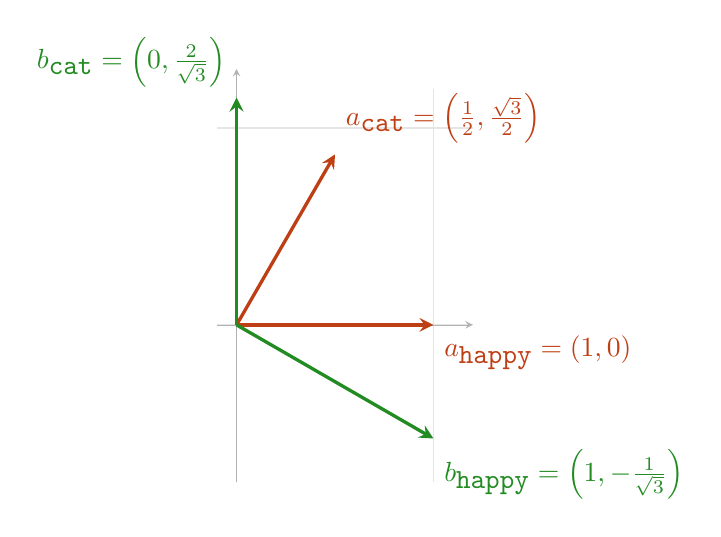
\begin{tikzpicture}[
    >=stealth,
    scale=2.5,
    vector/.style={->, very thick},
    axis/.style={very thin, gray!60},
    grid/.style={thin, gray!20}
]

\draw[grid] (-0.1,-0.8) grid (1.2,1.2);

\draw[axis,->] (-0.1,0) -- (1.2,0) node[right] {};
\draw[axis,->] (0,-0.8) -- (0,1.3) node[above] {};

\draw[vector,Bittersweet] (0,0) -- (0.5,0.866)
   node[above right] {$a_{\texttt{cat}} = \left(\frac{1}{2}, \frac{\sqrt{3}}{2}\right)$};

\draw[vector,Bittersweet] (0,0) -- (1,0)
   node[below right] {$a_{\texttt{happy}} = (1,0)$};

\draw[vector,ForestGreen] (0,0) -- (0,1.1547)
   node[above left] {$b_{\texttt{cat}} = \left(0, \frac{2}{\sqrt{3}}\right)$};

\draw[vector,ForestGreen] (0,0) -- (1,-0.577)
   node[below right] {$b_{\texttt{happy}} = \left(1, -\frac{1}{\sqrt{3}}\right)$};


\end{tikzpicture}
\caption{Representation vectors $a_{\texttt{cat}}, a_{\texttt{happy}}$ and probe vectors $b_{\texttt{cat}}, b_{\texttt{happy}}$ that yield perfect linear recovery of the \texttt{cat} and \texttt{happy} features. Notice that while the representation vectors are not orthogonal, the probe vectors are able perfectly extract features since the \texttt{cat} probe is orthogonal to the \texttt{happy} representation and the \texttt{happy} probe is orthogonal to the \texttt{cat} representation. Indeed, observe that $b_{\texttt{cat}}(z_{\texttt{cat}}a_{\texttt{cat}} + z_{\texttt{happy}}a_{\texttt{happy}}) = z_{\texttt{cat}}\langle b_{\texttt{cat}}, a_{\texttt{cat}}\rangle + z_{\texttt{happy}}\langle b_{\texttt{cat}}, a_{\texttt{happy}}\rangle = z_{\texttt{cat}}\cdot 1 + z_{\texttt{happy}}\cdot 0.$}
\end{figure}

\subsection{Contributions: Implications for the Linear Representation Hypothesis and the Theory of Language Models}

While linear representations have long been a central character in the empirical study of language models \citep{mikolov2013distributed,alain2016understanding}, it has been unclear whether the LRH can provide a theoretical basis by which to study language models. Here, we explore this possibility by providing mathematical foundations for the linear representation hypothesis. The framework we introduce provides definitional clarity on the LRH, cleanly distinguishing the distinct assumptions of linear representation and linear accessibility, and allowing us to formally consider the amount of superposition (i.e., the number of features stored relative to the number of neurons) possible under the LRH.

The framework allows us to then derive theoretical implications of the linear representation hypothesis. Mathematically, we establish a quantitative gap between compressed sensing and \textit{linear} compressed sensing. Our main results demonstrate dependencies between superposition (the number of features stored relative to the number of neurons), sparsity (the number of features active per input), accessibility (the precision by which the next layer can access features stored in the previous layer), and feature geometry (the arrangement of linear directions corresponding to features).
\end{ReviewVerbatim}

% report-context-presentation-sha256: d8b032ebd65c3bb868542352267ae4b19106bc80a0c63f83d3c5bd40414bc934
\paragraph{Settled source reading}
Lower bound: add ε < 1 to the printed condition on ε.

\paragraph{Expanded PaperInterface specification}
\begin{ReviewVerbatim}
∀ {epsilon : ℝ},
  0 < epsilon →
    epsilon < 1 →
      GKP26LinearRepresentationHypothesis.linearCompressedSensingLowerSourceLogScale =O[GKP26LinearRepresentationHypothesis.linearCompressedSensingLowerSourceFilter
          epsilon]
        fun (p : ℕ × ℕ) =>
        ↑(GKP26LinearRepresentationHypothesis.paper_linear_compressed_sensing_dimension p.1 p.2 epsilon)
\end{ReviewVerbatim}

\paragraph{Lean-elaborated claim roles}\begin{ReviewVerbatim}
1. parameter: ℝ
2. assumption: 0 < epsilon
3. assumption: epsilon < 1
4. conclusion: GKP26LinearRepresentationHypothesis.linearCompressedSensingLowerSourceLogScale =O[GKP26LinearRepresentationHypothesis.linearCompressedSensingLowerSourceFilter
    epsilon]
  fun (p : ℕ × ℕ) => ↑(GKP26LinearRepresentationHypothesis.paper_linear_compressed_sensing_dimension p.1 p.2 epsilon)
\end{ReviewVerbatim}

\paragraph{Lean proof endpoint (built separately)}\begin{ReviewVerbatim}
GKP26LinearRepresentationHypothesis.paper_lower_bound_dimension_isBigO_source_log_source_regime
\end{ReviewVerbatim}

\paragraph{Recorded source-to-Spec screening}
\textbf{Verdict:} \texttt{matches}
\\
{\raggedright
\textbf{Reason:} Compared the Lower Bound theorem at cited publication:\allowbreak{}220-\allowbreak{}227 and the supplied cited publication:\allowbreak{}327-\allowbreak{}380 context with the expanded target and all six supplied prerequisites, honoring LRH-\allowbreak{}LOWER-\allowbreak{}BOUND-\allowbreak{}NONDEGENERATE-\allowbreak{}EPSILON-\allowbreak{}01 only for this row.\allowbreak{} Epsilon is universally quantified outside the asymptotic assertion with 0 < epsilon < 1, so its Big-\allowbreak{}O constant may depend on epsilon, as in Omega\_\allowbreak{}epsilon.\allowbreak{} For p = (m,k), the displayed scale k\textasciicircum{}2*(log(m/\allowbreak{}k)/\allowbreak{}log(k)) is algebraically the printed (k\textasciicircum{}2/\allowbreak{}log(k))*log(m/\allowbreak{}k).\allowbreak{} The filter takes the joint natural-\allowbreak{}size limit restricted to 2 <= k and 5*k\textasciicircum{}3 < epsilon\textasciicircum{}2*m;\allowbreak{} its epsilon bounds are already supplied by the public hypotheses.\allowbreak{} Under positive epsilon and k >= 2, the squared strict inequality forces m > 0 and is equivalent to epsilon > sqrt(5)*k\textasciicircum{}(3/\allowbreak{}2)/\allowbreak{}sqrt(m).\allowbreak{} The k >= 2 condition holds eventually in this limit and avoids log(k) = 0.\allowbreak{} In the approved epsilon regime the inequality also gives m > k, making the displayed logarithmic scale positive;\allowbreak{} consequently scale =O dimension expresses the stated lower bound, not an upper bound on dimension.\allowbreak{} The dimension wrappers display a positive-\allowbreak{}epsilon minimum-\allowbreak{}dimension choice and the predicate requiring feasibility at d and d <= every feasible d';\allowbreak{} the nonpositive-\allowbreak{}epsilon fallback is outside this target.\allowbreak{} The source proof sketch discusses unrestricted representation and probe matrices, and none of these supplied target dependencies imposes A = B or an orthogonality restriction.\allowbreak{} This is an ordinary match under the approved epsilon clarification, not a corrected-\allowbreak{}target verdict.\allowbreak{}
\par}
\reviewmatch{Matches source input}
\noindent\textbf{Reviewer annotation}\par
\reviewerbox
\clearpage
\hypertarget{source-claim-5793edfccf93335e}{}
\section*{Review row 7}
\textbf{Source locator:} {\footnotesize\raggedright cited publication, lines 412-\allowbreak{}418\par}
\paragraph{Verbatim source input}
\begin{ReviewVerbatim}
\begin{lemma}[Incoherence of Random Matrices]\label{prop:incoherent}
    Let $C\in \RR^{d\times m}$ be a matrix with i.i.d. scaled Rademacher entries $\pm\frac{1}{\sqrt{d}}$. For
    \begin{equation}
        d = O\left(\frac{\log m + \log \frac{1}{\delta}}{\mu^2}\right),
    \end{equation}
    $C$ is $\mu$-incoherent with probability at least $1 - \delta$.
\end{lemma}
\end{ReviewVerbatim}



\paragraph{Expanded PaperInterface specification}
\begin{ReviewVerbatim}
∀ {m : ℕ} {mu delta : ℝ},
  2 ≤ m →
    0 < mu →
      0 < delta →
        delta ≤ 1 →
          ∃ (d : ℕ),
            0 < d ∧
              ↑d ≤ Real.log (2 * ↑m ^ 2 / delta) / (mu ^ 2 / 2) + 2 ∧
                (AppliedModelingLib.measureProb
                      (AppliedModelingLib.Probability.RademacherMatrix.rowsMeasure (Fin m) (Fin d))
                      fun (ω : Fin d → Fin m → Bool) =>
                      ∀ {{i j : Fin m}},
                        i ≠ j →
                          |AppliedModelingLib.Math.LinearCompressedSensing.inner
                                (AppliedModelingLib.Probability.RademacherMatrix.scaledMatrix ω i)
                                (AppliedModelingLib.Probability.RademacherMatrix.scaledMatrix ω j)| <
                            mu) ≥
                    1 - delta ∧
                  ∀ (ω : Fin d → Fin m → Bool) (i : Fin m),
                    AppliedModelingLib.Math.LinearCompressedSensing.inner
                        (AppliedModelingLib.Probability.RademacherMatrix.scaledMatrix ω i)
                        (AppliedModelingLib.Probability.RademacherMatrix.scaledMatrix ω i) =
                      1
\end{ReviewVerbatim}

\paragraph{Lean-elaborated claim roles}\begin{ReviewVerbatim}
1. parameter: ℕ
2. parameter: ℝ
3. parameter: ℝ
4. assumption: 2 ≤ m
5. assumption: 0 < mu
6. assumption: 0 < delta
7. assumption: delta ≤ 1
8. conclusion: ∃ (d : ℕ),
  0 < d ∧
    ↑d ≤ Real.log (2 * ↑m ^ 2 / delta) / (mu ^ 2 / 2) + 2 ∧
      (AppliedModelingLib.measureProb (AppliedModelingLib.Probability.RademacherMatrix.rowsMeasure (Fin m) (Fin d))
            fun (ω : Fin d → Fin m → Bool) =>
            ∀ {{i j : Fin m}},
              i ≠ j →
                |AppliedModelingLib.Math.LinearCompressedSensing.inner
                      (AppliedModelingLib.Probability.RademacherMatrix.scaledMatrix ω i)
                      (AppliedModelingLib.Probability.RademacherMatrix.scaledMatrix ω j)| <
                  mu) ≥
          1 - delta ∧
        ∀ (ω : Fin d → Fin m → Bool) (i : Fin m),
          AppliedModelingLib.Math.LinearCompressedSensing.inner
              (AppliedModelingLib.Probability.RademacherMatrix.scaledMatrix ω i)
              (AppliedModelingLib.Probability.RademacherMatrix.scaledMatrix ω i) =
            1
\end{ReviewVerbatim}

\paragraph{Lean proof endpoint (built separately)}\begin{ReviewVerbatim}
GKP26LinearRepresentationHypothesis.paper_random_rademacher_strict_incoherence_source_rate
\end{ReviewVerbatim}

\paragraph{Recorded source-to-Spec screening}
\textbf{Verdict:} \texttt{matches}
\\
{\raggedright
\textbf{Reason:} Under approved context LRH-\allowbreak{}RANDOM-\allowbreak{}INCOHERENCE-\allowbreak{}NONDEGENERATE-\allowbreak{}RANGE-\allowbreak{}01, the source lemma at cited publication:\allowbreak{}412-\allowbreak{}418 is read for m >= 2, mu > 0, and 0 < delta <= 1.\allowbreak{} The expanded target uses the i.\allowbreak{}i.\allowbreak{}d.\allowbreak{} scaled Rademacher row measure, gives an explicit d bounded by log(2*m\textasciicircum{}2/\allowbreak{}delta)/\allowbreak{}(mu\textasciicircum{}2/\allowbreak{}2)+2, proves probability at least 1-\allowbreak{}delta for strict off-\allowbreak{}diagonal incoherence, and records unit self-\allowbreak{}inner-\allowbreak{}products, matching the source rate and conclusion.\allowbreak{}
\par}
\reviewmatch{Matches source input}
\noindent\textbf{Reviewer annotation}\par
\reviewerbox
\clearpage
\hypertarget{source-claim-c333ecf427637954}{}
\section*{Review row 8}
\textbf{Source locator:} {\footnotesize\raggedright cited publication, lines 213-\allowbreak{}217\par}
\paragraph{Verbatim source input}
\begin{ReviewVerbatim}
\begin{theorem}[Upper Bound]\label{thm:upper}
    \begin{equation}
        d(m,k,\epsilon) = O_\epsilon\left(k^2\log m\right).
    \end{equation}
\end{theorem}

[Next verbatim source excerpt]

Taking $\mu = \frac{\epsilon}{k}$ and applying \Cref{prop:incoherent}, we have
\begin{equation}
    d(m,k,\epsilon) = O\left(\frac{k^2\log m}{\epsilon^2}\right),
\end{ReviewVerbatim}



\paragraph{Expanded PaperInterface specification}
\begin{ReviewVerbatim}
∀ {epsilon : ℝ},
  0 < epsilon →
    (fun (p : ℕ × ℕ) =>
        ↑(GKP26LinearRepresentationHypothesis.paper_linear_compressed_sensing_dimension p.1 p.2
            epsilon)) =O[Filter.atTop]
      fun (p : ℕ × ℕ) => ↑p.2 ^ 2 * Real.log ↑p.1
\end{ReviewVerbatim}

\paragraph{Lean-elaborated claim roles}\begin{ReviewVerbatim}
1. parameter: ℝ
2. assumption: 0 < epsilon
3. conclusion: (fun (p : ℕ × ℕ) =>
    ↑(GKP26LinearRepresentationHypothesis.paper_linear_compressed_sensing_dimension p.1 p.2 epsilon)) =O[Filter.atTop]
  fun (p : ℕ × ℕ) => ↑p.2 ^ 2 * Real.log ↑p.1
\end{ReviewVerbatim}

\paragraph{Lean proof endpoint (built separately)}\begin{ReviewVerbatim}
GKP26LinearRepresentationHypothesis.paper_upper_bound_dimension_isBigO_k_sq_log_m
\end{ReviewVerbatim}

\paragraph{Recorded source-to-Spec screening}
\textbf{Verdict:} \texttt{matches}
\\
{\raggedright
\textbf{Reason:} The source theorem at cited publication:\allowbreak{}213-\allowbreak{}217 and its displayed construction at lines 450-\allowbreak{}452 state d(m,k,epsilon) = O\_\allowbreak{}epsilon(k\textasciicircum{}2 log m).\allowbreak{} For each positive epsilon, the expanded target is exactly the minimum linear-\allowbreak{}compressed-\allowbreak{}sensing dimension IsBigO of k\textasciicircum{}2*log(m) at the product atTop filter, so the dependence, quantification, and conclusion agree.\allowbreak{}
\par}
\reviewmatch{Matches source input}
\noindent\textbf{Reviewer annotation}\par
\reviewerbox
\clearpage
\hypertarget{source-claim-b773a309f631cb95}{}
\section*{Review row 9}
\textbf{Source locator:} {\footnotesize\raggedright cited publication, lines 436\par}
\paragraph{Verbatim source input}
\begin{ReviewVerbatim}
In particular, the result guarantees the existence of a $\mu$-incoherent matrix with $d = O(\frac{\log m}{\mu^2}).$
\end{ReviewVerbatim}



\paragraph{Expanded PaperInterface specification}
\begin{ReviewVerbatim}
∀ {m : ℕ} {mu : ℝ},
  2 ≤ m →
    0 < mu →
      ∃ (d : ℕ) (A : GKP26LinearRepresentationHypothesis.paper_feature_matrix m d),
        ↑d ≤ 8 / mu ^ 2 * Real.log (2 * ↑m ^ 2) + 2 ∧
          GKP26LinearRepresentationHypothesis.paper_strict_mu_incoherent A mu
\end{ReviewVerbatim}

\paragraph{Lean-elaborated claim roles}\begin{ReviewVerbatim}
1. parameter: ℕ
2. parameter: ℝ
3. assumption: 2 ≤ m
4. assumption: 0 < mu
5. conclusion: ∃ (d : ℕ) (A : GKP26LinearRepresentationHypothesis.paper_feature_matrix m d),
  ↑d ≤ 8 / mu ^ 2 * Real.log (2 * ↑m ^ 2) + 2 ∧ GKP26LinearRepresentationHypothesis.paper_strict_mu_incoherent A mu
\end{ReviewVerbatim}

\paragraph{Lean proof endpoint (built separately)}\begin{ReviewVerbatim}
GKP26LinearRepresentationHypothesis.paper_rademacher_strict_incoherent_exists_source_rate
\end{ReviewVerbatim}

\paragraph{Recorded source-to-Spec screening}
\textbf{Verdict:} \texttt{matches}
\\
{\raggedright
\textbf{Reason:} The source prose at cited publication:\allowbreak{}436 asserts existence of a mu-\allowbreak{}incoherent d-\allowbreak{}by-\allowbreak{}m matrix with d = O(log m /\allowbreak{} mu\textasciicircum{}2).\allowbreak{} For m >= 2 and mu > 0, the expanded target supplies such a matrix, with unit self-\allowbreak{}inner-\allowbreak{}products and strict off-\allowbreak{}diagonal inner products below mu, and the explicit bound d <= (8/\allowbreak{}mu\textasciicircum{}2)*log(2*m\textasciicircum{}2)+2 has exactly the stated asymptotic rate.\allowbreak{}
\par}
\reviewmatch{Matches source input}
\noindent\textbf{Reviewer annotation}\par
\reviewerbox
\clearpage
\hypertarget{source-claim-b1fd683d79993219}{}
\section*{Review row 10}
\textbf{Source locator:} {\footnotesize\raggedright cited publication, lines 700-\allowbreak{}733\par}
\paragraph{Verbatim source input}
\begin{ReviewVerbatim}
Here, we prove that when feature representations are restricted to the Boolean cube $\{0,1\}^m,$ $\Omega(k^2\log (m/k))$ embedding dimensions are required to linearly separate embeddings with and without a feature. A corollary is that adding a bias and monotonic activation function does not increase the asymptotic capacity of embeddings.

\begin{theorem}\label{thm:threshold}
    Suppose that there exist $A,B \in \RR^{d\times m}$ and $t\in \RR^m$ such that for all $i\in [m]$ and $k$-sparse $z\in \{0,1\}^m$,
    \begin{equation}\label{eq:pineapple}
        (B^TAz)_i > t_i
    \end{equation}
    if and only if $z_i=1.$ Then for $k < \sqrt{m}$,
    \begin{equation}
        d = \Omega\left(\frac{k^2}{\log k}\log\frac{m}{k}\right).
    \end{equation}
\end{theorem}
It's worth noting here that taking $\epsilon < \frac{1}{2}$ in \Cref{thm:upper} provides a nearly-matching upper bound of $\Omega(k^2\log m)$, since $\epsilon < \frac{1}{2}$ implies that $(B^TAz)_i < \frac{1}{2}$ when $z_i = 0$ and $(B^TAz)_i > \frac{1}{2}$ when $z_i = 1$. Similarly, \Cref{thm:threshold} implies \Cref{thm:lower} in the case $\epsilon < \frac{1}{2}$. However, the lower bound in \Cref{thm:lower} does not directly imply \Cref{thm:threshold} since we do not require that $\norm{B^TAz - z}_\infty$ is small here, but rather that $Az$ linearly separates positive and negative examples for each feature. That being said, the proof is very similar to that of \Cref{thm:lower}, relying on the same overall strategy.

\begin{proof}
    Suppose that there existed $A,B\in \RR^{d\times m}$ and $t\in \RR^m$ such that for all $i\in [m]$ and $k$-sparse $z\in \{0,1\}^m,$ $(B^TAz)_i > t_i$ if and only if $z_i = 1.$ Then notice that we could scale the $i$-th column of $B$ and $\gamma_i$ by any constant positive factor to get another solution. In particular, we can obtain a solution where $B^TA$ is $1$ on the diagonal. Therefore, it suffices to show that for $d \le O(\frac{k^2}{\log k}\log \frac{m}{k}),$ there does not exist $B,A,t$ satisfying \eqref{eq:pineapple} and such that $(B^TA)_{ii} = 1$ for all $i\in [m].$

    Then we have that $t_i \le 1,$ since $(B^TAe_i) > t_i$ Then, along the lines of the proof of \Cref{thm:lower}, it suffices to find $i\in [m]$ and $T^*\subseteq [m]\setminus \{i\}$ with $|T^*|=2k$ and
    \begin{equation}
        |\langle b_i, a_j \rangle| > \frac{1}{k}
    \end{equation}
    for all $j\in T^*$. Indeed, this would imply the existence of a pair $i\in [m], T\subseteq [m]\setminus\{i\}$ (with $|T|=k$), such that
    \begin{equation}
        (B^TAz)_i > k\cdot \frac{1}{k} = 1 \ge t_i,
    \end{equation}
    giving a contradiction.

    We will again apply \Cref{lem:alon} to submatrices of $C$ of size $r$. Indeed, \Cref{lem:alon} implies that there exists a constant $\alpha > 0$ such that if $|R|=r$ and
    \begin{equation}
        \rank(C_R) < \alpha \frac{\log r}{(\frac{1}{k})^2\log k} = \alpha \frac{k^2}{\log k}\log r,
    \end{equation}
    then $C_R$ has an off-diagonal entry with absolute value at least $\frac{1}{k}.$ Then we can proceed as in the proof of \Cref{thm:lower}, taking $r = \frac{m}{4k+1}$ and applying Tur\'an's theorem.
\end{proof}
\end{ReviewVerbatim}



\paragraph{Expanded PaperInterface specification}
\begin{ReviewVerbatim}
GKP26LinearRepresentationHypothesis.thresholdActivationLowerSourceLogScale =O[GKP26LinearRepresentationHypothesis.thresholdActivationOriginalSourceFilter]
  fun (p : ℕ × ℕ) => ↑(GKP26LinearRepresentationHypothesis.thresholdSeparationDimension p.1 p.2)
\end{ReviewVerbatim}

\paragraph{Lean-elaborated claim roles}\begin{ReviewVerbatim}
1. conclusion: GKP26LinearRepresentationHypothesis.thresholdActivationLowerSourceLogScale =O[GKP26LinearRepresentationHypothesis.thresholdActivationOriginalSourceFilter]
  fun (p : ℕ × ℕ) => ↑(GKP26LinearRepresentationHypothesis.thresholdSeparationDimension p.1 p.2)
\end{ReviewVerbatim}

\paragraph{Lean proof endpoint (built separately)}\begin{ReviewVerbatim}
GKP26LinearRepresentationHypothesis.paper_threshold_separation_dimension_isBigO_lower_source_log_original_regime
\end{ReviewVerbatim}

\paragraph{Recorded source-to-Spec screening}
\textbf{Verdict:} \texttt{matches}
\\
{\raggedright
\textbf{Reason:} The theorem at cited publication:\allowbreak{}700-\allowbreak{}733 gives the threshold-\allowbreak{}separation lower bound k\textasciicircum{}2 log(m/\allowbreak{}k) /\allowbreak{} log(k) for k < sqrt(m).\allowbreak{} The expanded target expresses that Omega statement as the displayed source scale being IsBigO of the minimum threshold-\allowbreak{}separation dimension along the original-\allowbreak{}source-\allowbreak{}regime filter, and the supporting scale expands to exactly k\textasciicircum{}2 * (log(m/\allowbreak{}k) /\allowbreak{} log(k)).\allowbreak{}
\par}
\reviewmatch{Matches source input}
\noindent\textbf{Reviewer annotation}\par
\reviewerbox
\clearpage
\hypertarget{source-claim-331e1d36e419216b}{}
\section*{Review row 11}
\textbf{Source locator:} {\footnotesize\raggedright cited publication, lines 734-\allowbreak{}750\par}
\paragraph{Verbatim source input}
\begin{ReviewVerbatim}
The following corollary makes the simple observation that if a feature cannot be linearly separated, then it also cannot be separated by adding a bias and monotonic activation function.

\begin{corollary}\label{cor:activation-bias}
    Suppose that there exist $A,W \in \RR^{d\times m}$, $b\in \RR^m$, and a monotonically increasing activation function $\sigma:\RR\rightarrow \RR$ such that for all $i\in [m]$, $k$-sparse $z\in \{0,1\}^m$, and $x=Az,$
    \begin{equation}\label{eq:coconut}
        \sigma(W^Tx + b) > 0
    \end{equation}
    if and only if $z_i=1.$ (Here, $\sigma$ is applied component-wise.) Then for $k < \sqrt{m}$,
    \begin{equation}
        d = \Omega\left(\frac{k^2}{\log k}\log\frac{m}{k}\right).
    \end{equation}
\end{corollary}
\begin{proof}
    Consider any $i\in [m]$ and $z\in \{0,1\}^m$ such that $z_i = 1$ and $z'$ such that $z'_i = 0.$ Then $\sigma(W^TAz + b) > \sigma(W^TAz' + b).$ This implies that $(W^TAz)_i > (W^TAz')_i.$ Therefore, there exists a threshold $t_i$ such that for all $z\in \{0,1\}^m$, $(W^TAz)_i > t_i$ if and only if $z_i = 1$. The result follows by applying \Cref{thm:threshold}.
\end{proof}

The proof establishes that probes of the form $g_i(x) = \ReLU(W^Tx + b)$ implies the existence of a linear probe. In particular, this further establishes that for $\epsilon < \frac{1}{2}$, the bound in \Cref{thm:lower} cannot be lowered asymptotically by expanding the class of probes to allow a bias and activation function.
\end{ReviewVerbatim}



\paragraph{Expanded PaperInterface specification}
\begin{ReviewVerbatim}
GKP26LinearRepresentationHypothesis.thresholdActivationLowerSourceLogScale =O[GKP26LinearRepresentationHypothesis.thresholdActivationOriginalSourceFilter]
  fun (p : ℕ × ℕ) => ↑(GKP26LinearRepresentationHypothesis.activationSeparationDimension p.1 p.2)
\end{ReviewVerbatim}

\paragraph{Lean-elaborated claim roles}\begin{ReviewVerbatim}
1. conclusion: GKP26LinearRepresentationHypothesis.thresholdActivationLowerSourceLogScale =O[GKP26LinearRepresentationHypothesis.thresholdActivationOriginalSourceFilter]
  fun (p : ℕ × ℕ) => ↑(GKP26LinearRepresentationHypothesis.activationSeparationDimension p.1 p.2)
\end{ReviewVerbatim}

\paragraph{Lean proof endpoint (built separately)}\begin{ReviewVerbatim}
GKP26LinearRepresentationHypothesis.paper_activation_separation_dimension_isBigO_lower_source_log_original_regime
\end{ReviewVerbatim}

\paragraph{Recorded source-to-Spec screening}
\textbf{Verdict:} \texttt{matches}
\\
{\raggedright
\textbf{Reason:} The source corollary at cited publication:\allowbreak{}734-\allowbreak{}750 gives the k < sqrt(m) lower scale k\textasciicircum{}2 log(m/\allowbreak{}k) /\allowbreak{} log(k) for activation/\allowbreak{}bias separation.\allowbreak{} The expanded target expresses that Omega claim as the displayed source scale being IsBigO of the minimum activation-\allowbreak{}separation dimension along the displayed original-\allowbreak{}source-\allowbreak{}regime filter;\allowbreak{} the supporting scale has exactly k\textasciicircum{}2 * (log(m/\allowbreak{}k) /\allowbreak{} log(k)).\allowbreak{}
\par}
\reviewmatch{Matches source input}
\noindent\textbf{Reviewer annotation}\par
\reviewerbox

\end{document}
